\documentclass[10pt,xcolor=table]{beamer}

\usepackage{graphicx}
\usepackage{caption}
\usepackage{subcaption}
\usepackage{transparent}
 \usepackage{amsmath}
 
% \usepackage[utf8]{inputenc}
% \usepackage[T1]{fontenc}
\usepackage[table]{xcolor}    % loads also »colortbl« 
%  \usepackage{enumitem}
\usepackage{ucltemplate}
\usepackage{color}

\usepackage{pgfgantt} % for grantt charts
\usepackage{rotating}
\usepackage[graphicx]{realboxes}

\usepackage{tikz}
\usetikzlibrary{arrows,positioning, shapes.symbols,shapes.callouts,patterns,shapes,chains,calc,backgrounds,fadings}


\DeclareMathOperator*{\argmin}{arg\,min}
\DeclareMathOperator*{\argmax}{arg\,max}

% \definecolor{parCol}{rgb}{0.1, 0.1, 1}
% \definecolor{stCol}{rgb}{0.1, 0.6, 0.1}
% \definecolor{bothCol}{rgb}{0, 0.5, 0.5}

\definecolor{parCol}{rgb}{0, 0, 0}
\definecolor{stCol}{rgb}{0, 0, 0}
\definecolor{bothCol}{rgb}{0, 0, 0}
 
 %% UPGRADE PRESENTATION
%Information to be included in the title page:
\title{Disease Progression Analysis of typical Alzheimer’s Disease and Posterior Cortical Atrophy}
\author{Razvan Valentin Marinescu}
\institute{Center for Medical Image Computing, University College London}
\date{}

% logo of my university
\titlegraphic{
   \begin{figure}
   \begin{subfigure}{0.32\textwidth}
   \hspace{2em}
   
\includegraphics[height=1.0cm]{epsrc_logo.jpg}
   \end{subfigure}
   \begin{subfigure}{0.32\textwidth}
   \centering
   
\includegraphics[height=1.5cm]{NEWpond2017b.png} 
   \end{subfigure}
   \begin{subfigure}{0.32\textwidth}
   \centering
   
\includegraphics[height=1.0cm]{pondLogo.png} 
   \end{subfigure}
   
   \end{figure}
}
 
 
\setbeamersize{text margin left=15pt,text margin right=15pt,text margin bottom=15pt}


\begin{document}
 
\frame{\titlepage}
 
\setbeamerfont{frametitle}{size=\large}

% Presentation 9minutes in length + 3 min Q/A

\begin{frame}
\frametitle{Alzheimer's Disease}

\begin{itemize}
 \item The usual cause of dementia (60-70\% of cases)
 \item Symptoms: memory loss, problems with language, mood swings, loss of motivation
 \item Causes:
\end{itemize}

\vspace{-1em}
\begin{figure}
\centering
\begin{subfigure}{0.47\textwidth}
\centering
Genetics\\
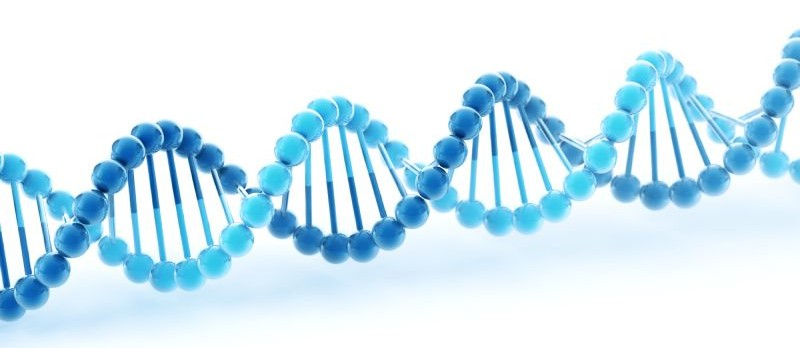
\includegraphics[scale=0.15]{DNA.jpg}
\end{subfigure}
\begin{subfigure}{0.47\textwidth}
\centering
Neurofibrillary tangles\\
\includegraphics[scale=0.07]{TANGLES_HIGH.jpg}
\end{subfigure}

\begin{subfigure}{0.47\textwidth}
\centering
\vspace{1em}
Amyloid-beta\\
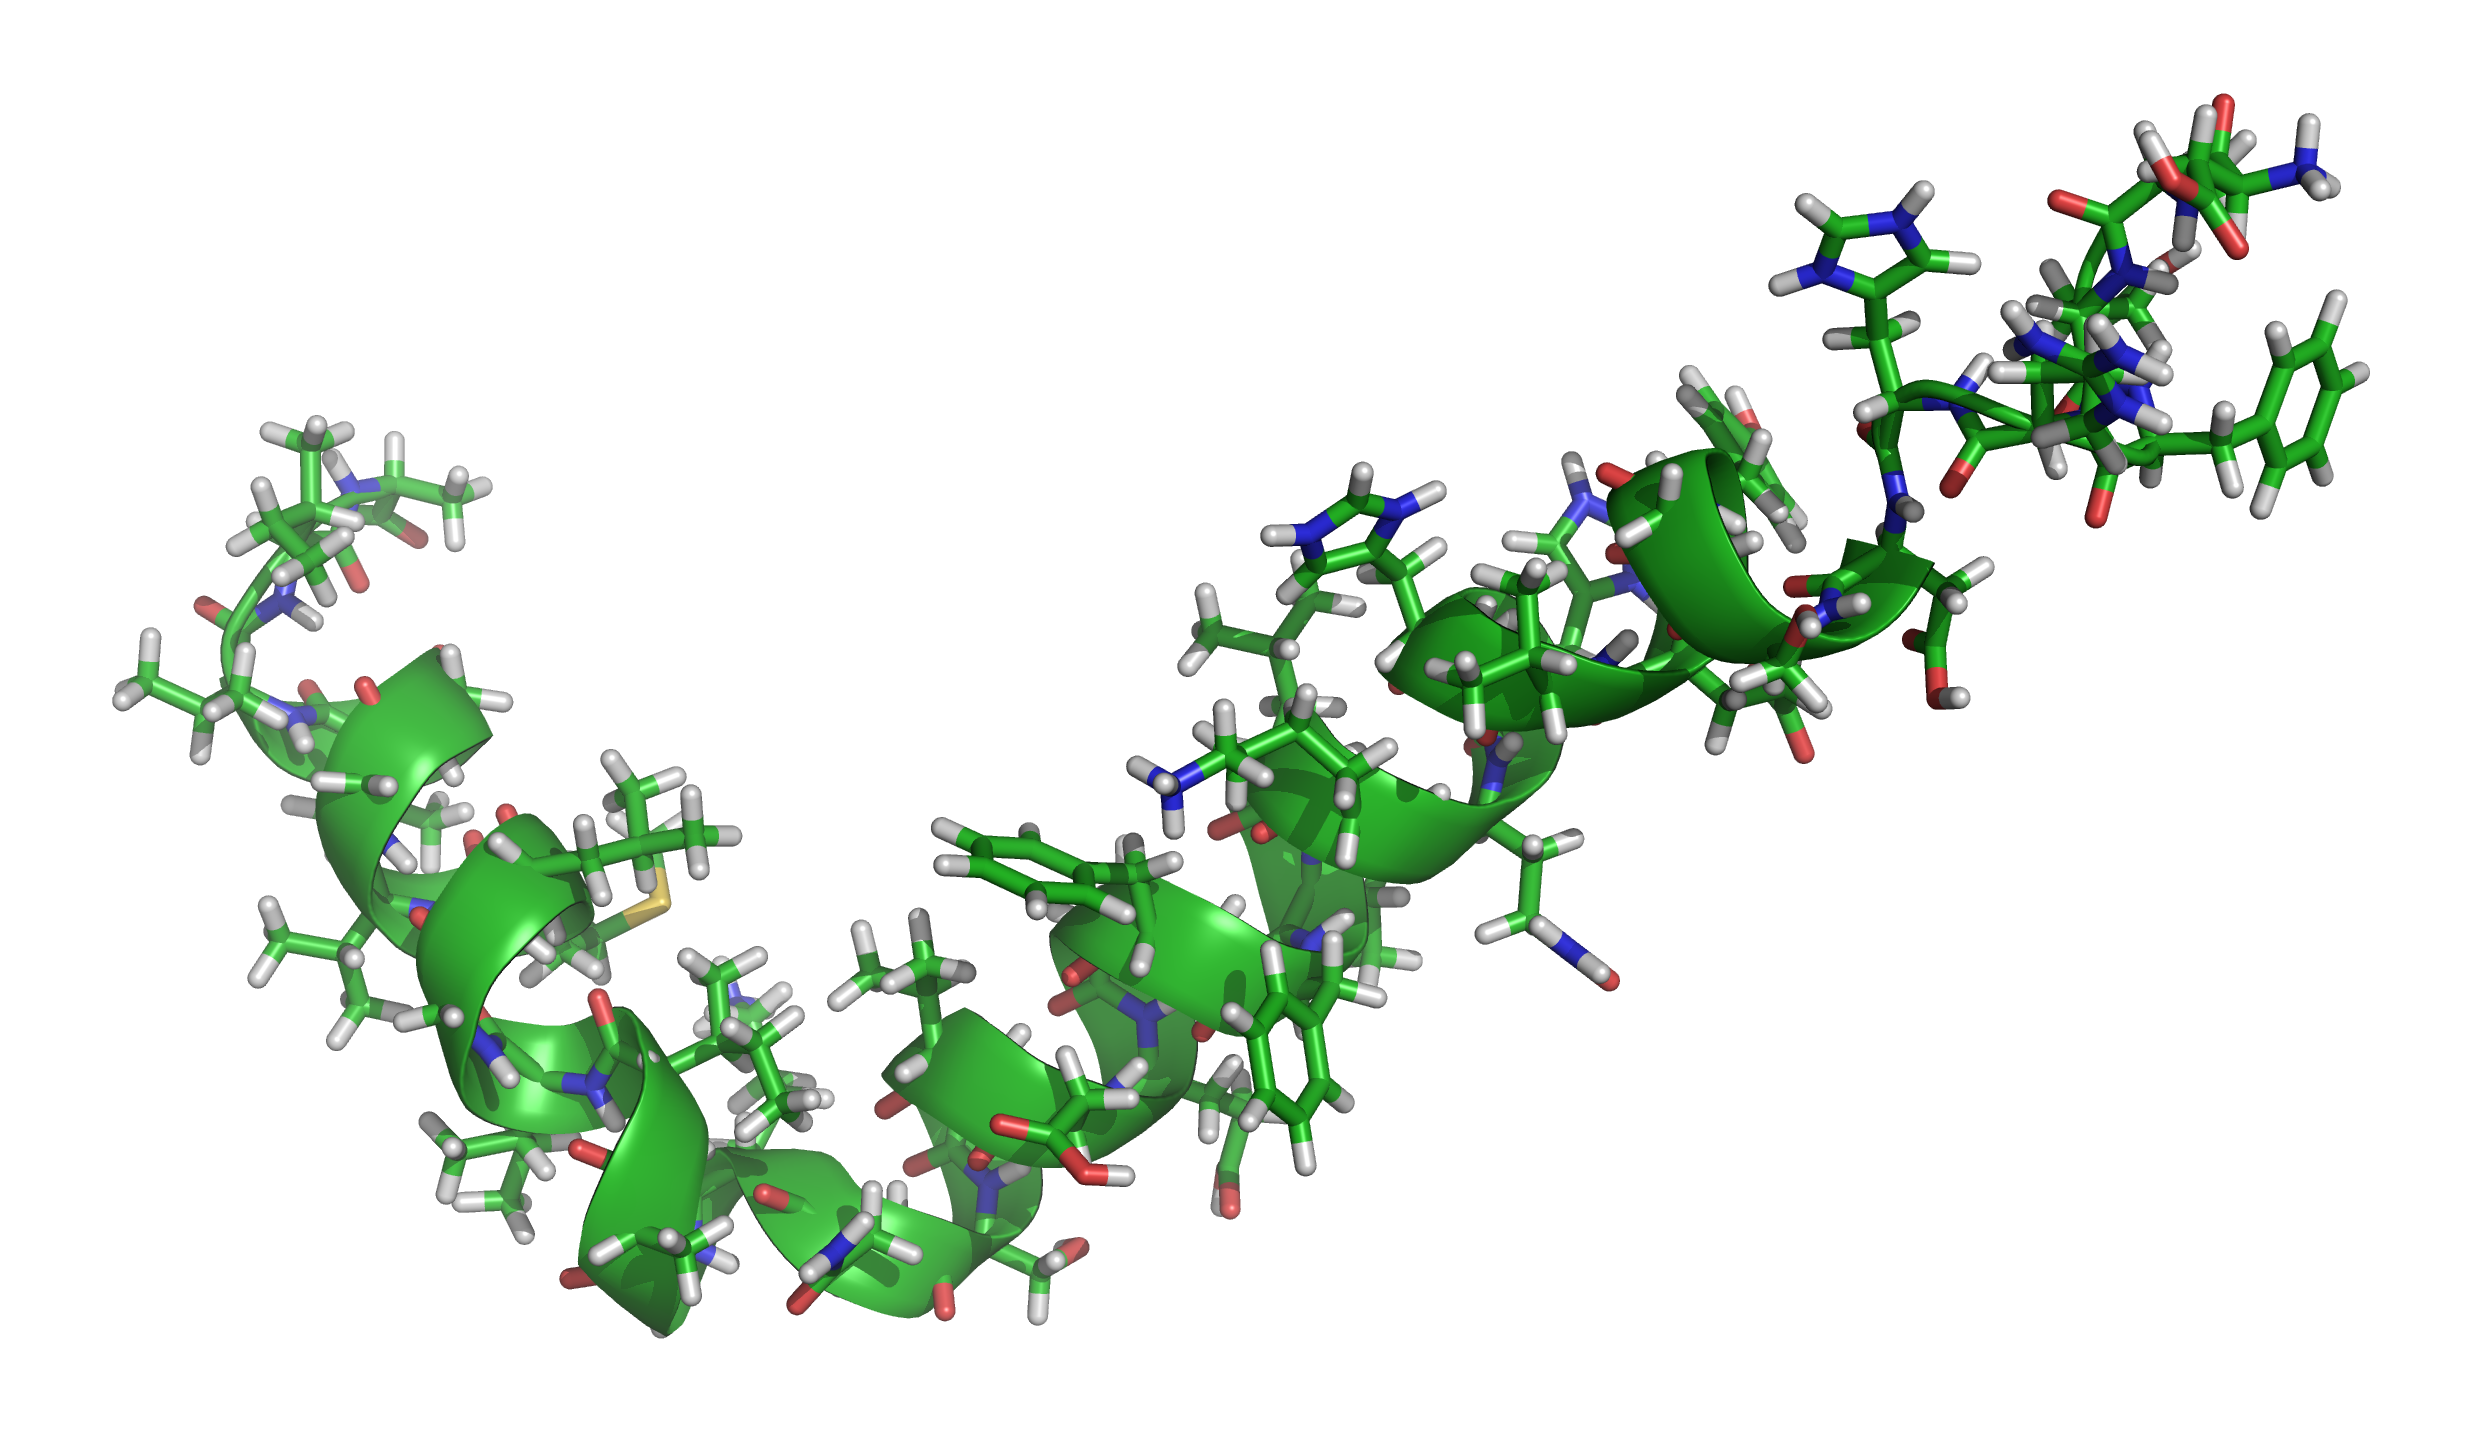
\includegraphics[scale=0.04]{amyloid_beta.png}
\end{subfigure}
\begin{subfigure}{0.47\textwidth}
\centering
\vspace{1em}
Vascular disease\\
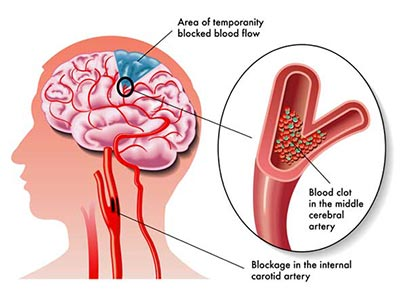
\includegraphics[scale=0.20]{vascular_disease.jpg}
\end{subfigure}

\end{figure}

\vspace{-1em}

\end{frame}

\begin{frame}
\frametitle{Posterior Cortical Atrophy}

% what is PCA
\textbf{Posterior Cortical Atrophy (PCA)}:
\begin{itemize}
 \item "Sub-type" of AD that affects the posterior part of the brain
 \item Symptoms: predominantly vision deficits
 \item Very rare: only 5\% of all AD cases 
\end{itemize}

\vspace{1em}
\begin{figure}
\centering 
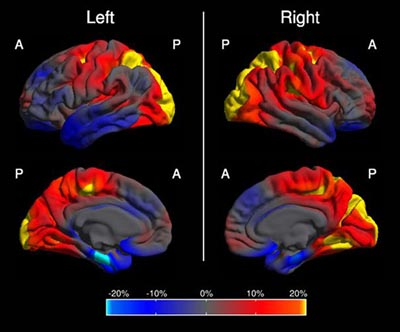
\includegraphics[scale=0.5]{PCAimageStory.jpg}
\end{figure}


\end{frame}

\begin{frame}
\frametitle{Disease progression modelling}
% explain what are the challenges

\begin{itemize}
 \item Builds a picture of the biomarker evolution across the disease timecourse
\end{itemize}


\begin{figure}
\centering 
\vspace{1em}
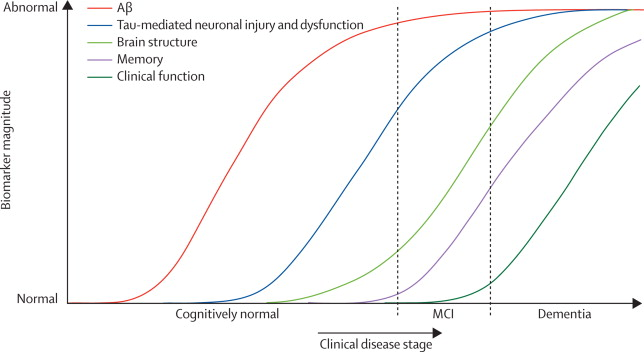
\includegraphics[scale=0.5]{jack_curves.jpg}
\end{figure}

% propose solutions
Building a picture of disease progression is challenging:
\begin{itemize}
 \item Patients are at different stages
 \item Biomarkers have different trajectories
 \item Cohort is heterogenous
\end{itemize}


\end{frame}


\begin{frame}
\frametitle{Project goals}

\begin{enumerate}
 \item Develop and improve disease progression models (DPMs)
 \item Study the progression of typical AD and PCA
%  \item Evaluate the performance of DPMs
\end{enumerate}

\end{frame}


\definecolor{light-gray}{gray}{0.6}

\begin{frame}
\frametitle{Contributions}
% summarize contributions

% \begin{itemize}
%   \item Applied the Event-Based Model (EBM) to tAD and PCA data
%   \item Applied the Differential Equation Model (DEM) to tAD and PCA data
%   \item Improved the EBM and DEM models and evaluated their performance
%   \item Developed a voxelwise disease progression model
% \end{itemize}

\vspace{-1em}
\begin{figure}
\centering
\begin{subfigure}{0.47\textwidth}
\centering
1. EBM modelling of PCA and tAD\\
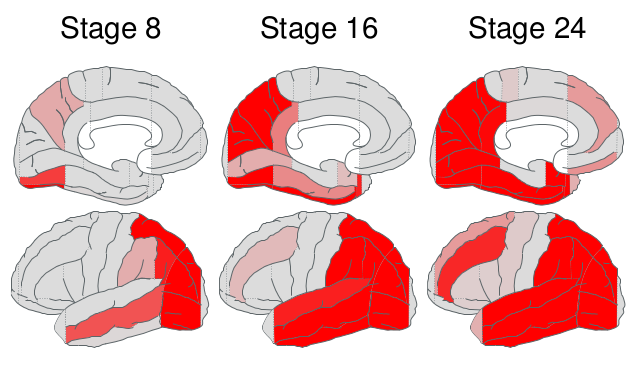
\includegraphics[scale=0.15]{ebm_thumb.png}
\end{subfigure}
\begin{subfigure}{0.47\textwidth}
\centering
2. DEM  modelling of PCA and tAD\\
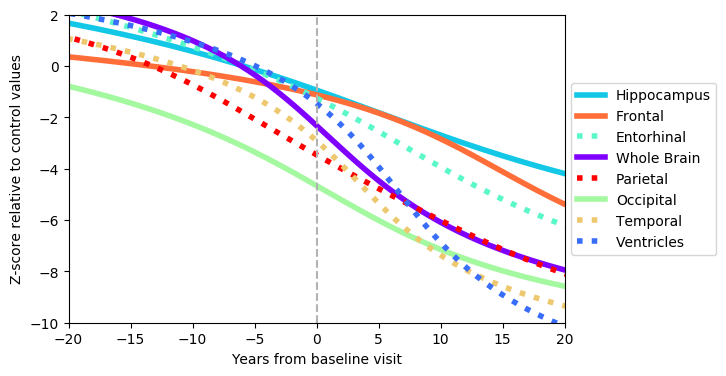
\includegraphics[scale=0.15]{../images/dem/mriSmallSebPaper_DEMStdPCA_trajAlign.png}
\end{subfigure}

\begin{subfigure}{0.47\textwidth}
\centering
3. Performance Evaluation of DPMs\\
\vspace{1em}
\resizebox{\columnwidth}{!}{%
 \begin{tabular}{c | c | c | c | c}
  Model & \multicolumn{2}{c |}{Staging Consistency} & \multicolumn{2}{c}{Time-lapse}\\
  & Hard & Soft & Hard & Soft\\
  
  \hline
  EBM - Standard & 0.91 $\pm$ 0.16 & 0.71 $\pm$ 0.07 & - & -\\
  \textbf{EBM - Sampling} & 0.96 $\pm$ 0.07 & 0.76 $\pm$ 0.10 & - & -\\
  \textbf{EBM - EM} & 0.99 $\pm$ 0.01 & 0.72 $\pm$ 0.07 & - & -\\
  DEM - Standard & 0.87 $\pm$ 0.10 & 0.88 $\pm$ 0.08 & 0.72 $\pm$ 0.91 & 0.67 $\pm$ 0.92\\
  \textbf{DEM - Optimised} & 0.87 $\pm$ 0.10 & 0.88 $\pm$ 0.08 & 0.74 $\pm$ 0.92 & 0.69 $\pm$ 0.92\\
  
 \end{tabular}
 }
\end{subfigure}
\begin{subfigure}{0.47\textwidth}
\centering
\vspace{2em}
4. Developed a Vertexwise Progression Model\\
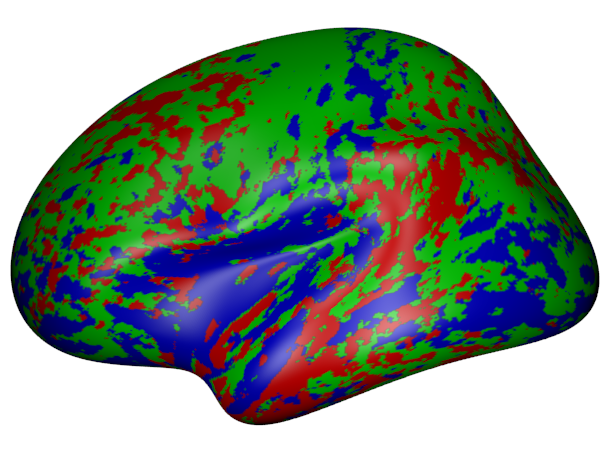
\includegraphics[width=0.5\columnwidth]{../images/vwdpm/blend14_adniThavgFWHM0InithistCl3Pr0Ra1_VWDPMStd.png}
\end{subfigure}

\end{figure}

\vspace{-1em}

% \vspace{1em}
% 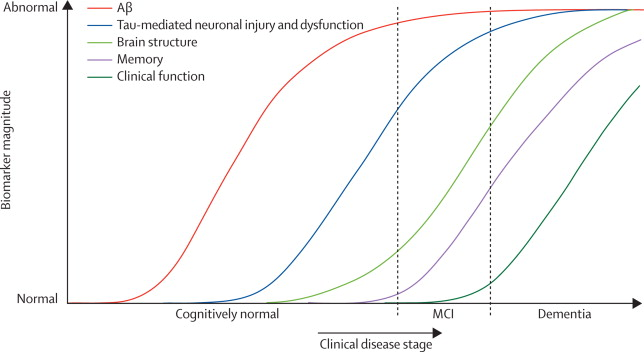
\includegraphics[scale=0.6]{jack_curves.jpg}

\end{frame}


\begin{frame}
\frametitle{Overview}
% summarize contributions

% \begin{itemize}
%   \item Applied the Event-Based Model (EBM) to tAD and PCA data
%   \item Applied the Differential Equation Model (DEM) to tAD and PCA data
%   \item Improved the EBM and DEM models and evaluated their performance
%   \item Developed a voxelwise disease progression model
% \end{itemize}

\vspace{-1em}
\begin{figure}
\centering
\begin{subfigure}{0.47\textwidth}
\centering

1. EBM modelling of PCA and tAD\\
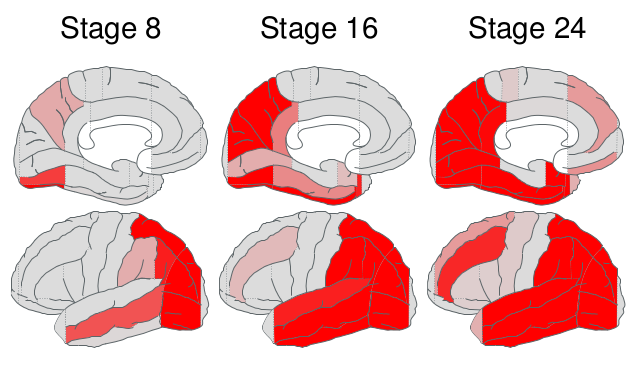
\includegraphics[scale=0.15]{ebm_thumb.png}

\end{subfigure}
\begin{subfigure}{0.47\textwidth}
\centering
{\transparent{0.4}
2. DEM  modelling of PCA and tAD\\
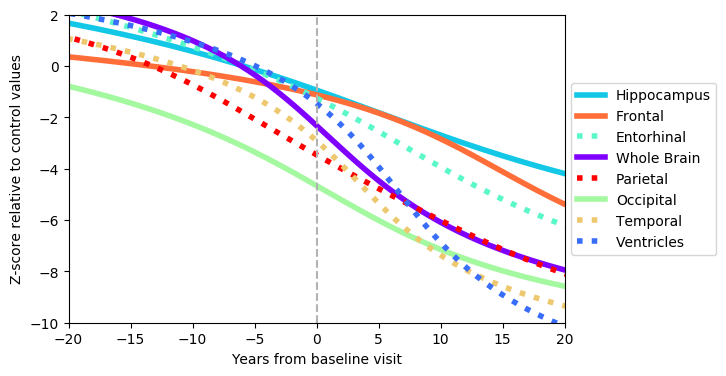
\includegraphics[scale=0.15]{../images/dem/mriSmallSebPaper_DEMStdPCA_trajAlign.png}
}
\end{subfigure}

\begin{subfigure}{0.47\textwidth}
\centering
{\transparent{0.4}
3. Performance Evaluation of DPMs\\
\vspace{1em}

\resizebox{\columnwidth}{!}{%
 \begin{tabular}{c | c | c | c | c}
  Model & \multicolumn{2}{c |}{Staging Consistency} & \multicolumn{2}{c}{Time-lapse}\\
  & Hard & Soft & Hard & Soft\\
  
  \hline
  EBM - Standard & 0.91 $\pm$ 0.16 & 0.71 $\pm$ 0.07 & - & -\\
  \textbf{EBM - Sampling} & 0.96 $\pm$ 0.07 & 0.76 $\pm$ 0.10 & - & -\\
  \textbf{EBM - EM} & 0.99 $\pm$ 0.01 & 0.72 $\pm$ 0.07 & - & -\\
  DEM - Standard & 0.87 $\pm$ 0.10 & 0.88 $\pm$ 0.08 & 0.72 $\pm$ 0.91 & 0.67 $\pm$ 0.92\\
  \textbf{DEM - Optimised} & 0.87 $\pm$ 0.10 & 0.88 $\pm$ 0.08 & 0.74 $\pm$ 0.92 & 0.69 $\pm$ 0.92\\
  
 \end{tabular}
 }
}
\end{subfigure}
\begin{subfigure}{0.47\textwidth}
\centering
\vspace{2em}
{\transparent{0.4}
4. Developed a Vertexwise Progression Model\\
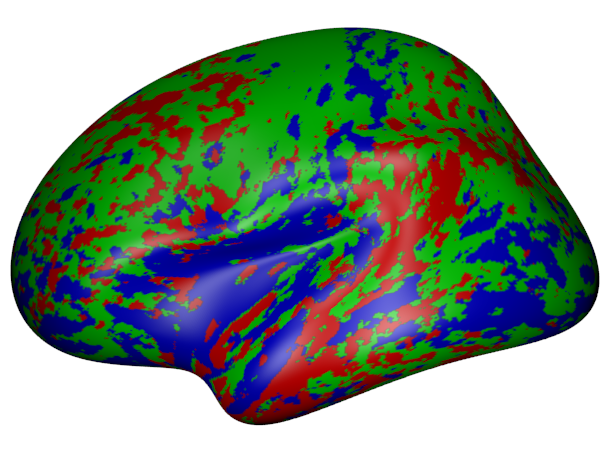
\includegraphics[width=0.5\columnwidth]{../images/vwdpm/blend14_adniThavgFWHM0InithistCl3Pr0Ra1_VWDPMStd.png}
}
\end{subfigure}

\end{figure}

\vspace{-1em}

% \vspace{1em}
% 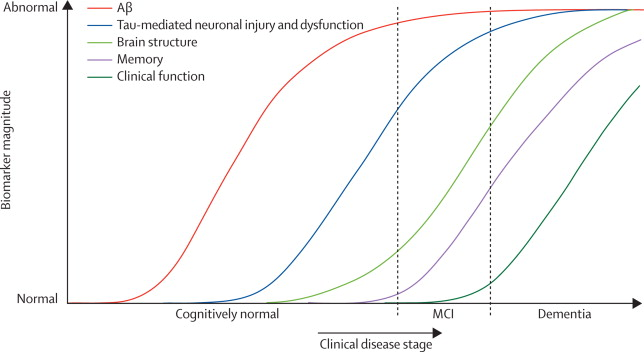
\includegraphics[scale=0.6]{jack_curves.jpg}

\end{frame}



\begin{frame}
\frametitle{Event-Based Model - PCA and tAD Analysis}
% discuss the hypotheses on PCA and tAD

\textbf{Clinical question}: Find the order in which brain regions become abnormal
\begin{itemize}
 \item in PCA 
 \item in tAD
\end{itemize}


\textbf{Methods}: Event-Based Model
\begin{itemize}
 \item Models atrophy progression as a sequence of abnormality events
 \item Estimates a distribution of normal and abnormal values for each biomarker
 \item Likelihood of abnormality sequence $S$:
 
\begin{equation}
\resizebox{0.8\columnwidth}{!}{% 
 $p(X|S) = \prod_{j=1}^J \left[ \sum_{k=0}^N p(k) \left( \prod_{i=1}^k p\left(x_{s(i),j} | E_{s(i)} \right) \prod_{i=k+1}^N p\left(x_{s(i),j} | \neg E_{s(i)}\right) \right) \right]$
 }
\end{equation}
\end{itemize}

\end{frame}


\newcommand*{\scaleBrainImg}{0.2}
\newcommand*{\scaleAllSubfigsImg}{0.4}
% scale parameter for the circles and the gradient
% \tikzset{every picture/.append style={scale=0.4}}

\newcommand*{\snapLocationPCA}{../images/ebm/mriAllGaussUnifDirPCA/snapshots} % or ../code/figures/mriAllGaussUnifDirPCA/snapshots

\begin{frame}
\frametitle{EBM - PCA Results}

{\scriptsize

\vspace{2em}

\definecolor{light-gray}{gray}{0.6}
\begin{figure}

  \begin{subfigure}{\textwidth}
  \centering
  %\begin{subfigure}[b]{0.15\textwidth}
    \begin{tikzpicture}[scale=\scaleAllSubfigsImg,auto,swap]

    % the two brain figures on top
    \node (upper_brain) at (0,1.5) { \includegraphics*[scale=\scaleBrainImg,trim=0 0 240 0,clip=true]{\snapLocationPCA/stage_8.eps}};
    \node (lower_brain) at (0,-1.5) { \includegraphics*[scale=\scaleBrainImg,trim=240 0 0 0,clip=true]{\snapLocationPCA/stage_8.eps}};
    \node[above=0cm of upper_brain] (stage) {Stage 8};
    % the balls
    
    \end{tikzpicture}
  %\end{subfigure}
  % next subfigure
  \hspace{-1.5em}
  ~
  %\begin{subfigure}[b]{0.15\textwidth}
    \begin{tikzpicture}[scale=\scaleAllSubfigsImg,auto,swap]

    % the two brain figures on top
    \node (upper_brain) at (0,1.5) { \includegraphics*[scale=\scaleBrainImg,trim=0 0 240 0,clip=true]{\snapLocationPCA/stage_16.eps}};
    \node (lower_brain) at (0,-1.5) { \includegraphics*[scale=\scaleBrainImg,trim=240 0 0 0,clip=true]{\snapLocationPCA/stage_16.eps}};
    \node[above=0cm of upper_brain] (stage) {Stage 16};
    % the balls
    
    \end{tikzpicture}
  %\end{subfigure}
  % next subfigure
  \hspace{-1.5em}
  ~
  %\begin{subfigure}[b]{0.15\textwidth}
    \begin{tikzpicture}[scale=\scaleAllSubfigsImg,auto,swap]

    % the two brain figures on top
    \node (upper_brain) at (0,1.5) { \includegraphics*[scale=\scaleBrainImg,trim=0 0 240 0,clip=true]{\snapLocationPCA/stage_24.eps}};
    \node (lower_brain) at (0,-1.5) { \includegraphics*[scale=\scaleBrainImg,trim=240 0 0 0,clip=true]{\snapLocationPCA/stage_24.eps}};
    \node[above=0cm of upper_brain] (stage) {Stage 24};
    % the balls
    
    \end{tikzpicture}
  %\end{subfigure}
  % next subfigure
  \hspace{-1.5em}
  ~
  %\begin{subfigure}[b]{0.15\textwidth}
    \begin{tikzpicture}[scale=\scaleAllSubfigsImg,auto,swap]

    % the two brain figures on top
    \node (upper_brain) at (0,1.5) { \includegraphics*[scale=\scaleBrainImg,trim=0 0 240 0,clip=true]{\snapLocationPCA/stage_32.eps}};
    \node (lower_brain) at (0,-1.5) { \includegraphics*[scale=\scaleBrainImg,trim=240 0 0 0,clip=true]{\snapLocationPCA/stage_32.eps}};
    \node[above=0cm of upper_brain] (stage) {Stage 32};
    % the balls
    
    \end{tikzpicture}
  %\end{subfigure}
  % next subfigure
  \hspace{-1.5em}
  ~
  %\begin{subfigure}[b]{0.15\textwidth}
    \begin{tikzpicture}[scale=\scaleAllSubfigsImg,auto,swap]

    % the two brain figures on top
    \node (upper_brain) at (0,1.5) { \includegraphics*[scale=\scaleBrainImg,trim=0 0 240 0,clip=true]{\snapLocationPCA/stage_40.eps}};
    \node (lower_brain) at (0,-1.5) { \includegraphics*[scale=\scaleBrainImg,trim=240 0 0 0,clip=true]{\snapLocationPCA/stage_40.eps}};
    \node[above=0cm of upper_brain] (stage) {Stage 40};
    % the balls
    
    \end{tikzpicture}
  %\end{subfigure}
  % next subfigure
  \hspace{-1.5em}
  ~
  \hspace{1em}
  % the red-to-yellow gradient on the right
  \begin{tikzpicture}[scale=\scaleAllSubfigsImg,auto,swap]
    \shade[top color=red,bottom color=gray!30] (0,0) rectangle (0.5,5);
    \node[inner sep=0] (corr_text) at (0.2,5.5) {abnormal};
    \node[inner sep=0] (corr_text) at (0.2,-0.5) {normal};
  \end{tikzpicture}
  \caption{Progression of brain volume loss}
%   \label{fig:SnapEBMPCAa}
  \end{subfigure}
  
  \begin{subfigure}{1\textwidth}
  \centering
  \includegraphics[scale=0.35]{\snapLocationPCA/../patientStages.eps}
  \caption{Subject staging}
%   \label{fig:SnapEBMPCAb}
  \end{subfigure}
  
\end{figure}

\par}

\end{frame}

\begin{frame}
\frametitle{EBM - Typical AD Results}

{\scriptsize


\newcommand*{\snapLocationAD}{../images/ebm/mriAllGaussUnifDirAD/snapshots} % or ../code/figures/mriAllGaussUnifDirPCA/snapshots

\vspace{2em}


\begin{figure}

  \begin{subfigure}{\textwidth}
  \centering
  %\begin{subfigure}[b]{0.15\textwidth}
    \begin{tikzpicture}[scale=\scaleAllSubfigsImg,auto,swap]

    % the two brain figures on top
    \node (upper_brain) at (0,1.5) { \includegraphics*[scale=\scaleBrainImg,trim=0 0 240 0,clip=true]{\snapLocationAD/stage_8.eps}};
    \node (lower_brain) at (0,-1.5) { \includegraphics*[scale=\scaleBrainImg,trim=240 0 0 0,clip=true]{\snapLocationAD/stage_8.eps}};
    \node[above=0cm of upper_brain] (stage) {Stage 8};
    % the balls
    
    \end{tikzpicture}
  %\end{subfigure}
  % next subfigure
  \hspace{-1.5em}
  ~
  %\begin{subfigure}[b]{0.15\textwidth}
    \begin{tikzpicture}[scale=\scaleAllSubfigsImg,auto,swap]

    % the two brain figures on top
    \node (upper_brain) at (0,1.5) { \includegraphics*[scale=\scaleBrainImg,trim=0 0 240 0,clip=true]{\snapLocationAD/stage_16.eps}};
    \node (lower_brain) at (0,-1.5) { \includegraphics*[scale=\scaleBrainImg,trim=240 0 0 0,clip=true]{\snapLocationAD/stage_16.eps}};
    \node[above=0cm of upper_brain] (stage) {Stage 16};
    % the balls
    
    \end{tikzpicture}
  %\end{subfigure}
  % next subfigure
  \hspace{-1.5em}
  ~
  %\begin{subfigure}[b]{0.15\textwidth}
    \begin{tikzpicture}[scale=\scaleAllSubfigsImg,auto,swap]

    % the two brain figures on top
    \node (upper_brain) at (0,1.5) { \includegraphics*[scale=\scaleBrainImg,trim=0 0 240 0,clip=true]{\snapLocationAD/stage_24.eps}};
    \node (lower_brain) at (0,-1.5) { \includegraphics*[scale=\scaleBrainImg,trim=240 0 0 0,clip=true]{\snapLocationAD/stage_24.eps}};
    \node[above=0cm of upper_brain] (stage) {Stage 24};
    % the balls
    
    \end{tikzpicture}
  %\end{subfigure}
  % next subfigure
  \hspace{-1.5em}
  ~
  %\begin{subfigure}[b]{0.15\textwidth}
    \begin{tikzpicture}[scale=\scaleAllSubfigsImg,auto,swap]

    % the two brain figures on top
    \node (upper_brain) at (0,1.5) { \includegraphics*[scale=\scaleBrainImg,trim=0 0 240 0,clip=true]{\snapLocationAD/stage_32.eps}};
    \node (lower_brain) at (0,-1.5) { \includegraphics*[scale=\scaleBrainImg,trim=240 0 0 0,clip=true]{\snapLocationAD/stage_32.eps}};
    \node[above=0cm of upper_brain] (stage) {Stage 32};
    % the balls
    
    \end{tikzpicture}
  %\end{subfigure}
  % next subfigure
  \hspace{-1.5em}
  ~
  %\begin{subfigure}[b]{0.15\textwidth}
    \begin{tikzpicture}[scale=\scaleAllSubfigsImg,auto,swap]

    % the two brain figures on top
    \node (upper_brain) at (0,1.5) { \includegraphics*[scale=\scaleBrainImg,trim=0 0 240 0,clip=true]{\snapLocationAD/stage_40.eps}};
    \node (lower_brain) at (0,-1.5) { \includegraphics*[scale=\scaleBrainImg,trim=240 0 0 0,clip=true]{\snapLocationAD/stage_40.eps}};
    \node[above=0cm of upper_brain] (stage) {Stage 40};
    % the balls
    
    \end{tikzpicture}
  %\end{subfigure}
  % next subfigure
  \hspace{-1.5em}
  ~
  \hspace{1em}
  % the red-to-yellow gradient on the right
  \begin{tikzpicture}[scale=\scaleAllSubfigsImg,auto,swap]
    \shade[top color=red,bottom color=gray!30] (0,0) rectangle (0.5,5);
    \node[inner sep=0] (corr_text) at (0.2,5.5) {abnormal};
    \node[inner sep=0] (corr_text) at (0.2,-0.5) {normal};
  \end{tikzpicture}
  \caption{Progression of brain volume loss}
%   \label{fig:SnapEBMPCAa}
  \end{subfigure}
  
  \begin{subfigure}{1\textwidth}
  \centering
  \includegraphics[scale=0.35]{\snapLocationAD/../patientStages.eps}
  \caption{Subject staging}
%   \label{fig:SnapEBMPCAb}
  \end{subfigure}
  
\end{figure}

\par}

\end{frame}

\makeatletter
\define@key{Gin}{pcaSubFigParams}[]{\setkeys{Gin}{trim=0 440 0 0,clip,scale=0.13}}
\makeatother

\begin{frame}
\frametitle{EBM - PCA Subtypes - Results}
% EAR, PER and SPE

% {\scriptsize

\begin{figure}
  \centering
 \begin{subfigure}{0.6\textwidth}
  \includegraphics[pcaSubFigParams]{../../docs/2017/aaic2017/figures/ebmImagesEAR.png}
 \end{subfigure}
 \begin{subfigure}{0.3\textwidth}
 \centering
 \scriptsize{\textbf{Vision subgroup}\\ (Visual impairment)}
 \end{subfigure}

  \begin{subfigure}{0.6\textwidth}
  \includegraphics[pcaSubFigParams]{../../docs/2017/aaic2017/figures/ebmImagesSPA.png}
 \end{subfigure}
  \begin{subfigure}{0.3\textwidth}
  \centering
 \scriptsize{\textbf{Space subgroup}\\ (Visuo-spatial impairment)}
 \end{subfigure}
 
 \begin{subfigure}{0.6\textwidth}
  \includegraphics[pcaSubFigParams]{../../docs/2017/aaic2017/figures/ebmImagesPER.png}
 \end{subfigure}
  \begin{subfigure}{0.3\textwidth}
  \centering
 \scriptsize{\textbf{Object subgroup}\\ (Visuo-perceptual impairment)}
 \end{subfigure}
 
% \par} 
 
\end{figure}

\end{frame}

\newcommand{\semitransp}[2][35]{\color{fg!#1}#2}


\begin{frame}
\frametitle{Overview}

\vspace{-1em}
\begin{figure}
\centering
\begin{subfigure}{0.47\textwidth}
\centering
{\transparent{0.4}
1. EBM modelling of PCA and tAD\\
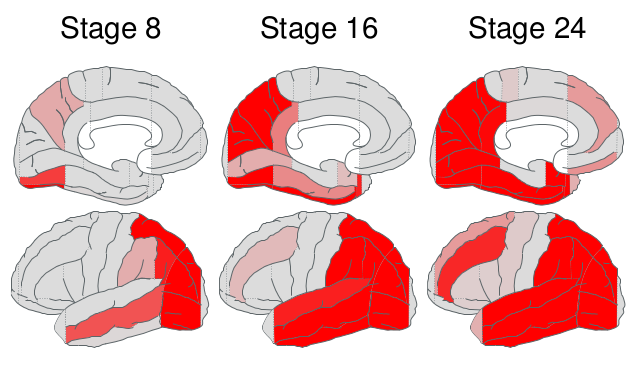
\includegraphics[scale=0.15]{ebm_thumb.png}
}
\end{subfigure}
\begin{subfigure}{0.47\textwidth}
\centering

2. DEM  modelling of PCA and tAD\\
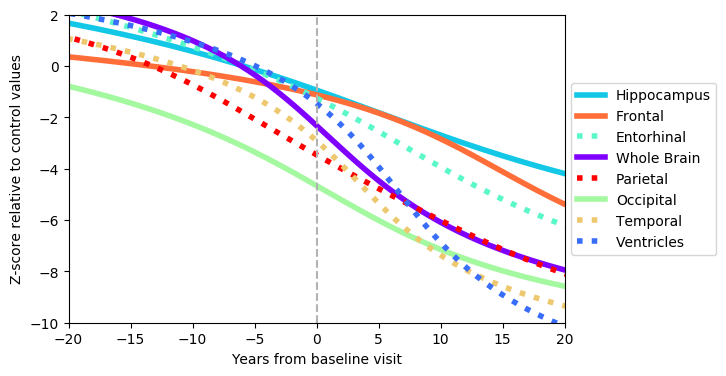
\includegraphics[scale=0.15]{../images/dem/mriSmallSebPaper_DEMStdPCA_trajAlign.png}

\end{subfigure}

\begin{subfigure}{0.47\textwidth}
\centering
{\transparent{0.4}
3. Performance Evaluation of DPMs\\
\vspace{1em}

\resizebox{\columnwidth}{!}{%
 \begin{tabular}{c | c | c | c | c}
  Model & \multicolumn{2}{c |}{Staging Consistency} & \multicolumn{2}{c}{Time-lapse}\\
  & Hard & Soft & Hard & Soft\\
  
  \hline
  EBM - Standard & 0.91 $\pm$ 0.16 & 0.71 $\pm$ 0.07 & - & -\\
  \textbf{EBM - Sampling} & 0.96 $\pm$ 0.07 & 0.76 $\pm$ 0.10 & - & -\\
  \textbf{EBM - EM} & 0.99 $\pm$ 0.01 & 0.72 $\pm$ 0.07 & - & -\\
  DEM - Standard & 0.87 $\pm$ 0.10 & 0.88 $\pm$ 0.08 & 0.72 $\pm$ 0.91 & 0.67 $\pm$ 0.92\\
  \textbf{DEM - Optimised} & 0.87 $\pm$ 0.10 & 0.88 $\pm$ 0.08 & 0.74 $\pm$ 0.92 & 0.69 $\pm$ 0.92\\
  
 \end{tabular}
 }
}
\end{subfigure}
\begin{subfigure}{0.47\textwidth}
\centering
\vspace{2em}
{\transparent{0.4}
4. Vertexwise Progression Model\\
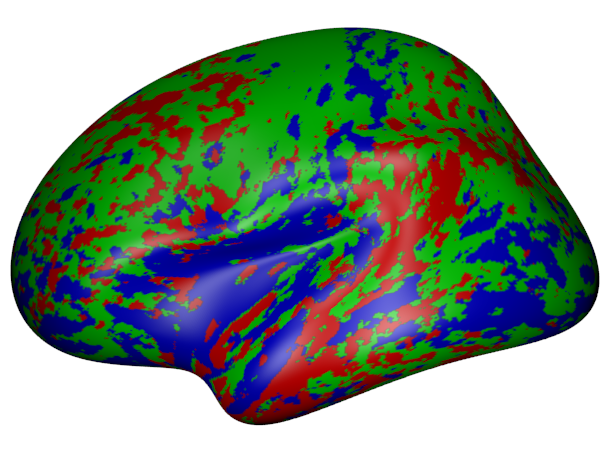
\includegraphics[width=0.5\columnwidth]{../images/vwdpm/blend14_adniThavgFWHM0InithistCl3Pr0Ra1_VWDPMStd.png}
}
\end{subfigure}

\end{figure}

\vspace{-1em}

% \vspace{1em}
% 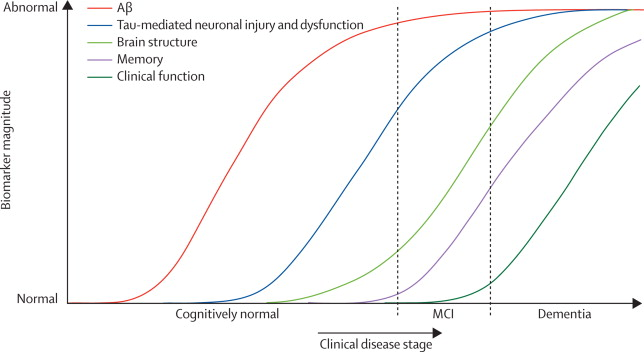
\includegraphics[scale=0.6]{jack_curves.jpg}

\end{frame}



\begin{frame}
\frametitle{Differential Equation Model - Clinical Questions}

We want to find the \textbf{timing}, \textbf{rate} and \textbf{extent} of atrophy:
\begin{itemize}
\item for the whole brain
\item across different brain regions 
\item in PCA compared to AD 
\end{itemize}

\textbf{Methods}:
\begin{itemize}
 \item We used a Differential Equation Model (DEM)
\end{itemize}


\end{frame}

\begin{frame}
\frametitle{DEM - Methods}
% Talk about the DEM

\newcommand{\figScale}{0.27}

\begin{figure}[H]
 \centering
 \begin{subfigure}{0.47\textwidth}
    \centering
    1. Fit linear subject-wise trajectories
    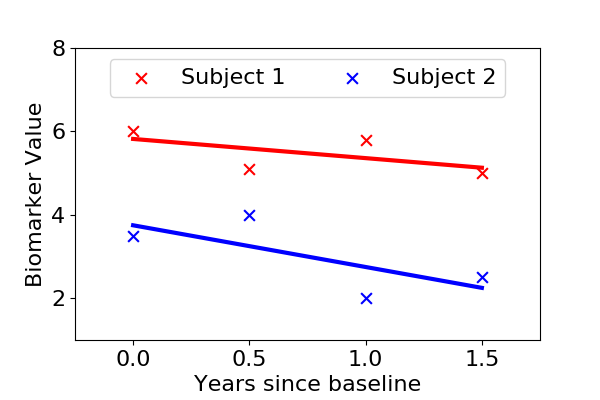
\includegraphics[scale=\figScale]{fig1_linReg.png}
%     \caption{}
    \vspace{1em}
 \end{subfigure}
 \begin{subfigure}{0.47\textwidth}
     \centering
     2. Fit rate of change model using GPs\\
     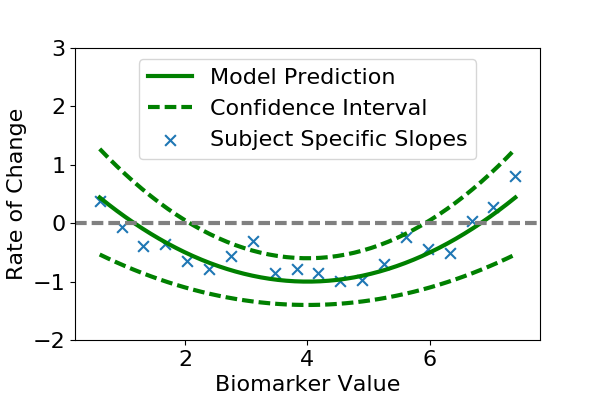
\includegraphics[scale=\figScale]{fig2_GP.png}
%      \caption{}
     \vspace{1em}
 \end{subfigure}
 
  \begin{subfigure}{0.47\textwidth}
    \centering
    3. Integrate rate of change model\\
    \vspace{0.7em}
    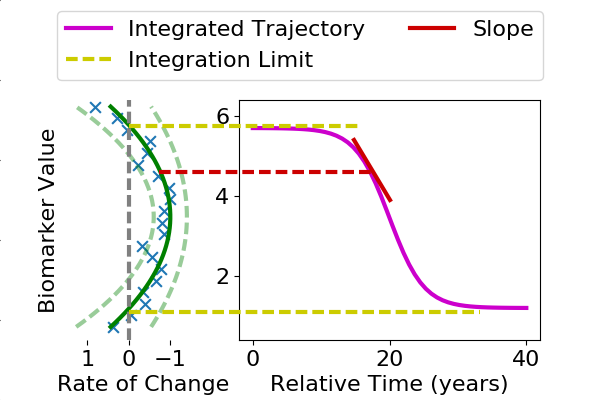
\includegraphics[scale=\figScale]{fig3_recon.png}
%     \caption{}
 \end{subfigure}
 \begin{subfigure}{0.47\textwidth}
     \centering
     4. Align the trajectories on the temporal axis
     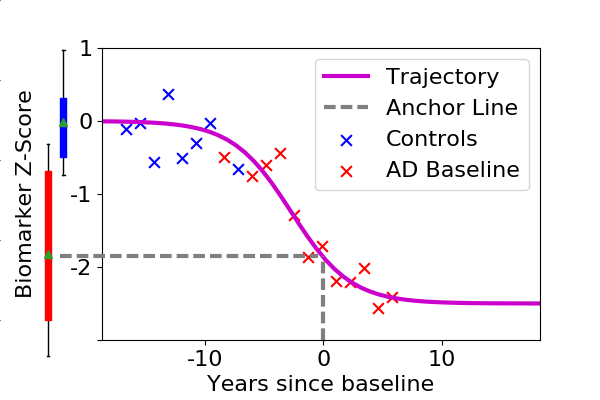
\includegraphics[scale=\figScale]{fig4_align.png}
%      \caption{}
 \end{subfigure}
\end{figure}

\end{frame}

\begin{frame}
\frametitle{DEM - Results - PCA and tAD}


Progression of brain volume loss using the differential equation model:

\begin{figure}
\hspace{-0.5em}
\begin{subfigure}{0.47\textwidth}
 \centering
%  \hspace{-2.5cm}
 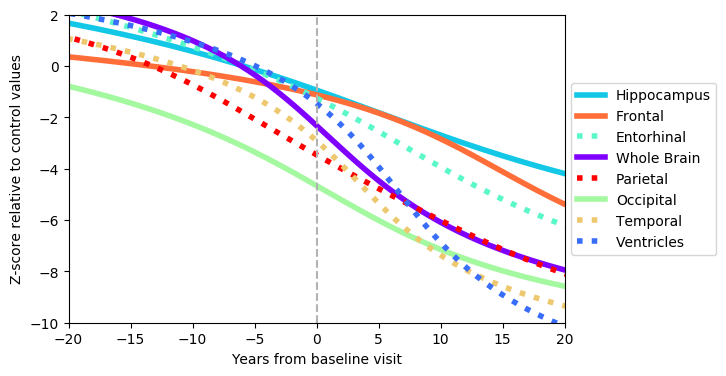
\includegraphics[scale=0.3]{../images/dem/mriSmallSebPaper_DEMStdPCA_trajAlign.png}
 \caption{PCA}
 \label{fig:trajDEMPCA}
\end{subfigure}
\hspace{1em}
\begin{subfigure}{0.47\textwidth}
 \centering
%  \hspace{-2.5cm}
 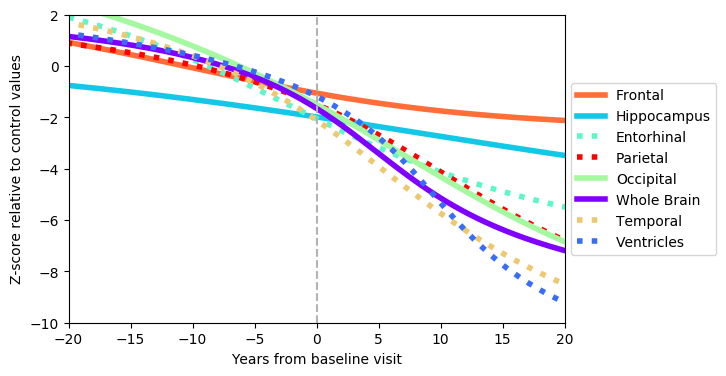
\includegraphics[scale=0.3]{../images/dem/mriSmallSebPaper_DEMStdAD_trajAlign.png}
 \caption{tAD}
  \label{fig:trajDEMAD}
\end{subfigure}
% \label{fig:trajDEM}
\end{figure}

\end{frame}

\begin{frame}
\frametitle{DEM - PCA vs tAD Progression across ROIs}


\begin{figure}
%  \centering
 \hspace{-1cm}
 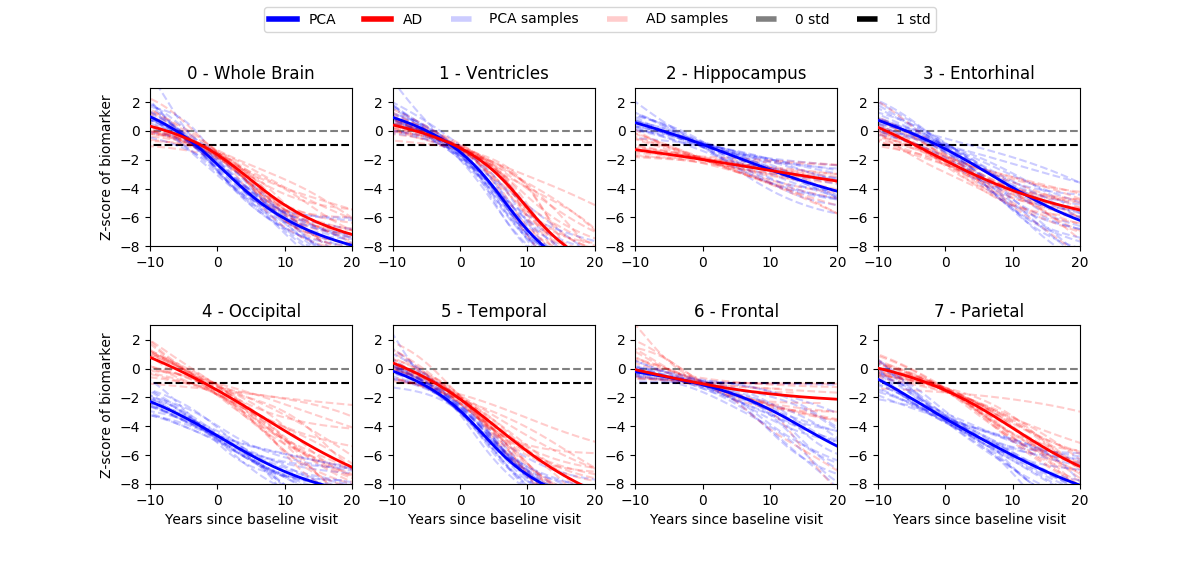
\includegraphics[scale=0.33, trim=0 0 0 30,clip=true]{../images/dem/mriSmallSebPaper_DEMStd_subplotsPcaAd.png}
%  \caption{}
 \label{trajDEMPcaAd}
\end{figure}

\textbf{Conclusion}: 
\begin{itemize}
 \item In tAD, the hippocampus and entorhinal areas become abnormal earlier
 \item In PCA, the occipital and parietal regions becomes abnormal earlier
\end{itemize}


\end{frame}

\begin{frame}
\frametitle{Overview}

\vspace{-1em}
\begin{figure}
\centering
\begin{subfigure}{0.47\textwidth}
\centering
{\transparent{0.4}
1. EBM modelling of PCA and tAD\\
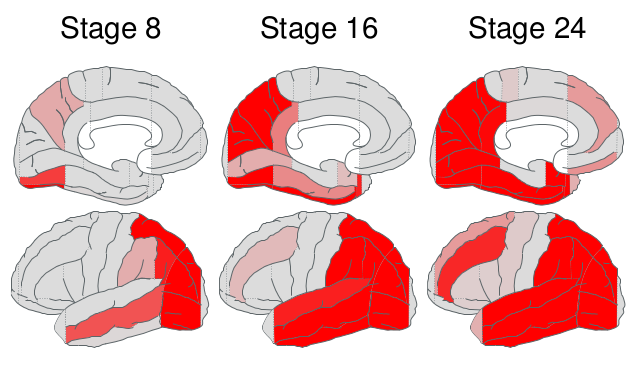
\includegraphics[scale=0.15]{ebm_thumb.png}
}
\end{subfigure}
\begin{subfigure}{0.47\textwidth}
\centering
{\transparent{0.4}
2. DEM  modelling of PCA and tAD\\
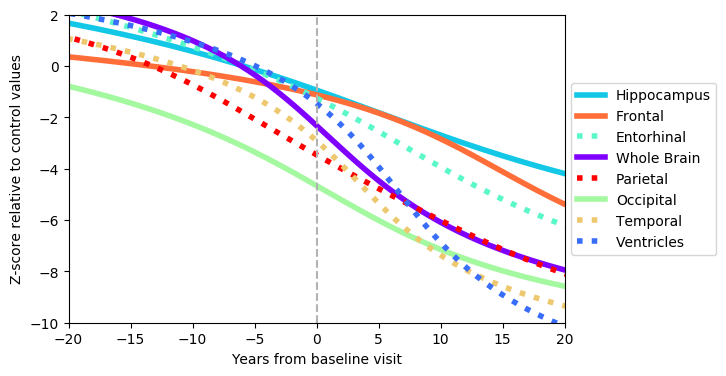
\includegraphics[scale=0.15]{../images/dem/mriSmallSebPaper_DEMStdPCA_trajAlign.png}
}
\end{subfigure}

\begin{subfigure}{0.47\textwidth}
\centering

3. Performance Evaluation of DPMs\\
\vspace{1em}

\resizebox{\columnwidth}{!}{%
 \begin{tabular}{c | c | c | c | c}
  Model & \multicolumn{2}{c |}{Staging Consistency} & \multicolumn{2}{c}{Time-lapse}\\
  & Hard & Soft & Hard & Soft\\
  
  \hline
  EBM - Standard & 0.91 $\pm$ 0.16 & 0.71 $\pm$ 0.07 & - & -\\
  \textbf{EBM - Sampling} & 0.96 $\pm$ 0.07 & 0.76 $\pm$ 0.10 & - & -\\
  \textbf{EBM - EM} & 0.99 $\pm$ 0.01 & 0.72 $\pm$ 0.07 & - & -\\
  DEM - Standard & 0.87 $\pm$ 0.10 & 0.88 $\pm$ 0.08 & 0.72 $\pm$ 0.91 & 0.67 $\pm$ 0.92\\
  \textbf{DEM - Optimised} & 0.87 $\pm$ 0.10 & 0.88 $\pm$ 0.08 & 0.74 $\pm$ 0.92 & 0.69 $\pm$ 0.92\\
  
 \end{tabular}
 }

\end{subfigure}
\begin{subfigure}{0.47\textwidth}
\centering
\vspace{2em}
{\transparent{0.4}
4. Vertexwise Progression Model\\
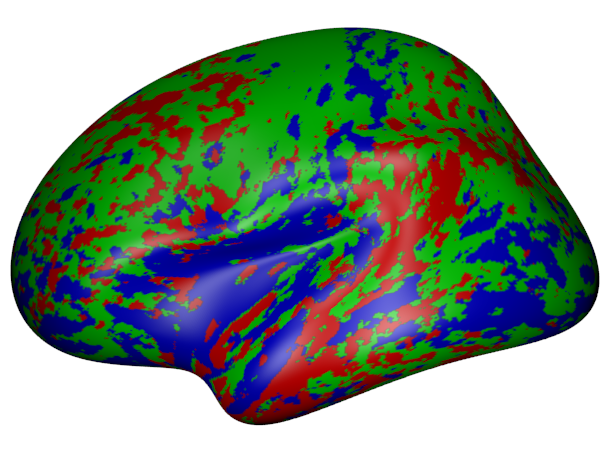
\includegraphics[width=0.5\columnwidth]{../images/vwdpm/blend14_adniThavgFWHM0InithistCl3Pr0Ra1_VWDPMStd.png}
}
\end{subfigure}

\end{figure}

\vspace{-1em}

% \vspace{1em}
% 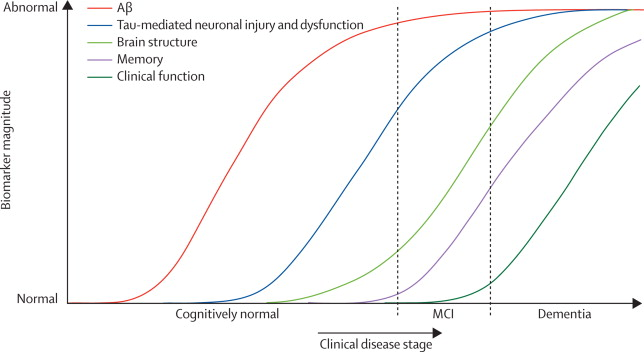
\includegraphics[scale=0.6]{jack_curves.jpg}

\end{frame}

\begin{frame}
\frametitle{Performance Evaluation - Aims}

\textbf{Aims}\\
Evaluate the performance of:
\begin{itemize}
 \item different disease progression models
 \item different fitting procedures
\end{itemize}

\textbf{Methods}\\
\begin{itemize}
 \item Implemented improved fitting procedures for EBM (2 methods) and DEM (1 method)
 \item Tested if the improved fitting procedures perform better
 \item Performed the evaluation on two datasets: ADNI and DRC
\end{itemize}

\end{frame}

\begin{frame}
\frametitle{EBM Improvement 1 - Blocked MCMC}

Devised a novel EBM fitting procedure:
\begin{itemize}
 \item Optimises both the sequence and event distribution parameters simultaneously
 \item Uses a blocked MCMC sampling algorithm
 \item Convergence is slower
 \item Parameters sampled are  $\theta_j = [S_j^{new}, \mu^n_j, \sigma^n_j, \mu^a_j, \sigma^a_j]$, where:
\end{itemize}

$$p(X|S, [\mu^n_j, \sigma^n_j, \mu^a_j, \sigma^a_j]^{j=1 \dots N}) = $$

\vspace{-1em}
$$ \prod_{i=1}^P \left[ \sum_{k=0}^N p(k) \left( \prod_{j=1}^k p\left(x_{i,S(i)} | \mu^a_{S(j)}, \sigma^a_{S(j)} \right) \prod_{j=k+1}^N p\left(x_{i,S(j)} | \mu^n_{S(j)}, \sigma^n_{S(j)} \right) \right) \right]
$$

\end{frame}

\begin{frame}
\frametitle{EBM Improvement 2 - Expectation Maximisation}

\begin{itemize}
 \item More efficient parameter estimation for the EBM using the EM framework
 \item \textbf{E-step}: Update subject stages
 \vspace{-0.5em}
 $$ Q(\theta | \theta^{old}) = \sum_{z_1, \dots, z_P}  p(Z = z_1, \dots, z_P |X, \theta^{old})\ \sum_{i=1}^{P}$$

$$  \left[ \sum_{j=1}^{z_i} log\ N(x_{ij}|\mu_{S(j)}^a, \sigma_{S(j)}^a) + \sum_{j=z_i + 1}^N log\ N(x_{ij}|\mu_{S(j)}^n, \sigma_{S(j)}^n) \right] $$

 \item \textbf{M-step}: Update the distribution paramerters and sequence. 
 \end{itemize}
 \vspace{-0.5em}
 $$ \mu_k^n = \sum_{i=1}^P x_{ik} w_i^n$$

$$w_i^n = \frac{p(S^{-1}(k) > Z_i | X, \theta^{old})}{\sum_{i=1}^P \ p(S^{-1}(k) > Z_i | X, \theta^{old})}$$

\end{frame}


\begin{frame}
\frametitle{DEM Improvement - Temporal Alignment of Trajectories}

\begin{itemize}
 \item More efficient temporal alignment of trajectories
 \item For each trajectory $f_b$ we estimate:
 \begin{itemize}
  \item a temporal shift $t_i$
  \item a measurement noise $\sigma_i$
 \end{itemize}
 \item Full model likelihood is:
\end{itemize}

 
$$ p(X| t_1, \dots, t_B, \sigma_1, \dots , \sigma_B) = \prod_{p=1}^{P} \sum_{z_p} p(Z_p = z_p) \prod_{b=1}^{B}  N(x_{pb}|f_b(z_p-t_b), \sigma_b)$$

\begin{itemize}
 \item where:
\begin{itemize}
 \item $Z_p$ is the stage of patient $p$ 
 \item $x_{pb}$ is the value of patient $p$ for biomarker $b$
\end{itemize}
\end{itemize}


\end{frame}



\begin{frame}
\frametitle{Performance Evaluation - Results}

\vspace{2em}

{\small


{\scriptsize

% staging metrics - PCA
\begin{table}[ht]
\centering
 \begin{tabular}{c | c | c | c | c}
  Model & \multicolumn{2}{c |}{Staging Consistency} & \multicolumn{2}{c}{Time-lapse}\\
  & Hard & Soft & Hard & Soft\\
  
  \hline
  EBM - Standard & 0.88 $\pm$ 0.12 & 0.66 $\pm$ 0.09 & - & -\\ 
  \textbf{EBM - Sampling} & 0.96 $\pm$ 0.06 & 0.70 $\pm$ 0.06  & - & - \par\\
  \textbf{EBM - EM} & 0.95 $\pm$ 0.10 & 0.68 $\pm$ 0.11 & - & -\\
  DEM - Standard & 0.94 $\pm$ 0.06 & 0.95 $\pm$ 0.05 & 0.54 $\pm$ 0.31 & 0.52 $\pm$ 0.29\\
  \textbf{DEM - Optimised} & 0.95 $\pm$ 0.05 & 0.95 $\pm$ 0.04 & 0.56 $\pm$ 0.28 & 0.52 $\pm$ 0.27\\
  
 \end{tabular}
 \caption{PCA - DRC cohort}
 \label{tab:drcStagingResPCA}
\end{table}

\par}


{\scriptsize

% staging metrics - AD
\begin{table}[ht]
\centering
 \begin{tabular}{c | c | c | c | c}
  Model & \multicolumn{2}{c |}{Staging Consistency} & \multicolumn{2}{c}{Time-lapse}\\
  & Hard & Soft & Hard & Soft\\
  
  \hline
  EBM - Standard & 0.91 $\pm$ 0.16 & 0.71 $\pm$ 0.07 & - & -\\
  \textbf{EBM - Sampling} & 0.96 $\pm$ 0.07 & 0.76 $\pm$ 0.10 & - & -\\
  \textbf{EBM - EM} & 0.99 $\pm$ 0.01 & 0.72 $\pm$ 0.07 & - & -\\
  DEM - Standard & 0.87 $\pm$ 0.10 & 0.88 $\pm$ 0.08 & 0.72 $\pm$ 0.91 & 0.67 $\pm$ 0.92\\
  \textbf{DEM - Optimised} & 0.87 $\pm$ 0.10 & 0.88 $\pm$ 0.08 & 0.74 $\pm$ 0.92 & 0.69 $\pm$ 0.92\\
  
 \end{tabular}
 \caption{tAD - DRC cohort}
 \label{tab:drcStagingResAD}
\end{table}

\par}

\textbf{Conclusion}: Novel methods generally perform better than the standard methods.

}
\vspace{2em}

\end{frame}

\begin{frame}
\frametitle{Overview}

\vspace{-1em}
\begin{figure}
\centering
\begin{subfigure}{0.47\textwidth}
\centering
{\transparent{0.4}
1. EBM modelling of PCA and tAD\\
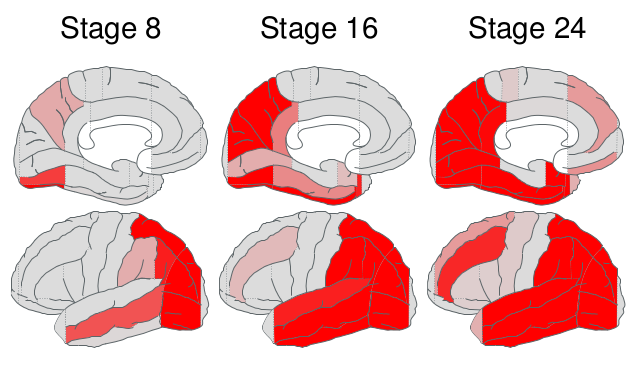
\includegraphics[scale=0.15]{ebm_thumb.png}
}
\end{subfigure}
\begin{subfigure}{0.47\textwidth}
\centering
{\transparent{0.4}
2. DEM  modelling of PCA and tAD\\
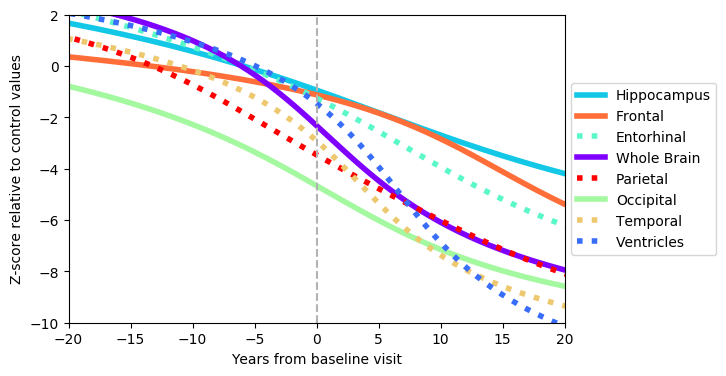
\includegraphics[scale=0.15]{../images/dem/mriSmallSebPaper_DEMStdPCA_trajAlign.png}
}
\end{subfigure}

\begin{subfigure}{0.47\textwidth}
\centering
{\transparent{0.4}
3. Performance Evaluation of DPMs\\
\vspace{1em}

\resizebox{\columnwidth}{!}{%
 \begin{tabular}{c | c | c | c | c}
  Model & \multicolumn{2}{c |}{Staging Consistency} & \multicolumn{2}{c}{Time-lapse}\\
  & Hard & Soft & Hard & Soft\\
  
  \hline
  EBM - Standard & 0.91 $\pm$ 0.16 & 0.71 $\pm$ 0.07 & - & -\\
  \textbf{EBM - Sampling} & 0.96 $\pm$ 0.07 & 0.76 $\pm$ 0.10 & - & -\\
  \textbf{EBM - EM} & 0.99 $\pm$ 0.01 & 0.72 $\pm$ 0.07 & - & -\\
  DEM - Standard & 0.87 $\pm$ 0.10 & 0.88 $\pm$ 0.08 & 0.72 $\pm$ 0.91 & 0.67 $\pm$ 0.92\\
  \textbf{DEM - Optimised} & 0.87 $\pm$ 0.10 & 0.88 $\pm$ 0.08 & 0.74 $\pm$ 0.92 & 0.69 $\pm$ 0.92\\
  
 \end{tabular}
 }
}
\end{subfigure}
\begin{subfigure}{0.47\textwidth}
\centering
\vspace{2em}

4. Vertexwise Progression Model\\
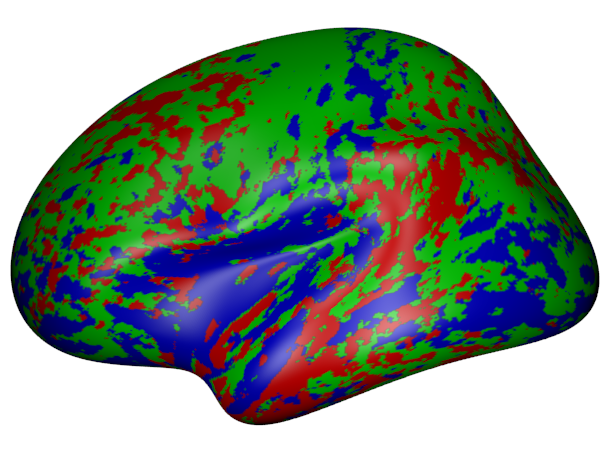
\includegraphics[width=0.5\columnwidth]{../images/vwdpm/blend14_adniThavgFWHM0InithistCl3Pr0Ra1_VWDPMStd.png}

\end{subfigure}

\end{figure}

\vspace{-1em}

% \vspace{1em}
% 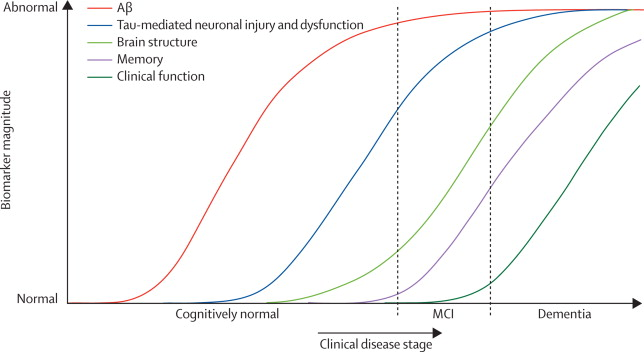
\includegraphics[scale=0.6]{jack_curves.jpg}

\end{frame}

\begin{frame}
\frametitle{Vertexwise Disease Progression Model (VDPM)}

\vspace{-3em}
\textbf{Idea}:
\begin{itemize}
 \item Use vertexwise measures of cortical thickness
 \item Consider each vertex measurement as a "biomarker"
 \item Estimate a fine-grained spatial distribution of atrophy 
  \begin{itemize}
  \item without a-priori defined ROIs
 \end{itemize}
\end{itemize}
\textbf{Motivation}:
\begin{itemize}
 \item Information is lost when averaging all voxel measures within an ROI.
 \item Atrophy patterns correlate with functional networks, which are not spatially connected (Seeley et al., 2009)
\end{itemize}

\vspace{-1em}

\begin{figure}
\centering
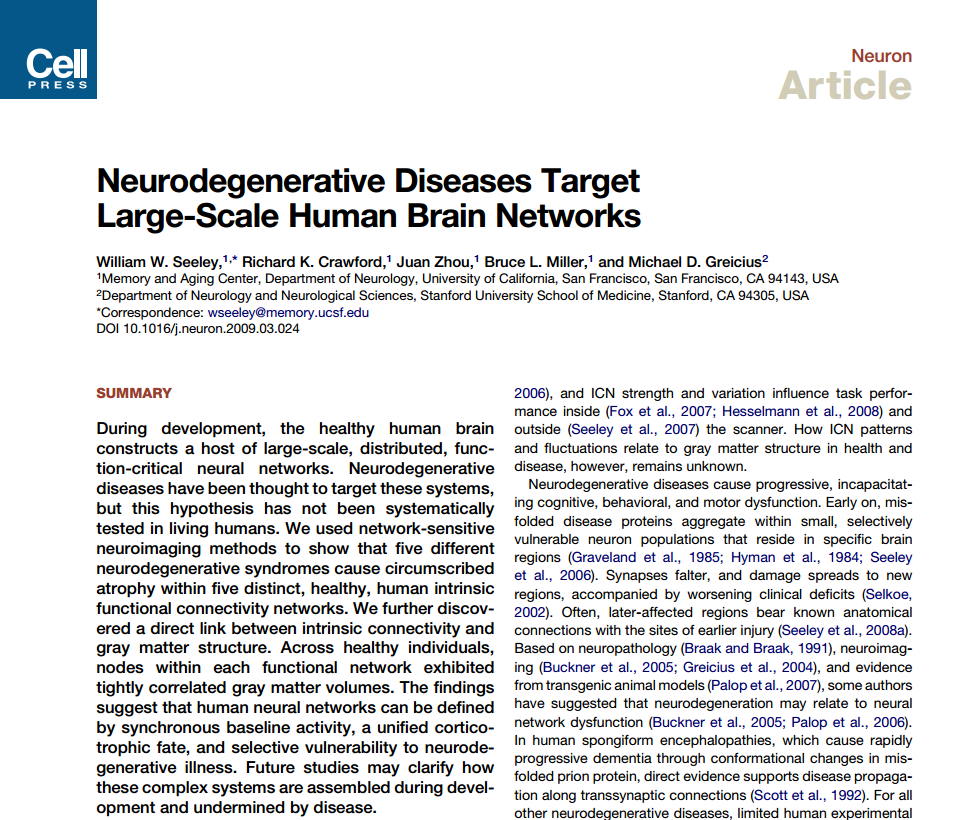
\includegraphics[scale=0.3, trim= 0 800 0 0]{seeley.png}
\end{figure}



\end{frame}


\begin{frame}
\frametitle{Vertexwise Model - Method}

\newcommand{\lw}{0.5mm}
% \newcommand{\mycirc}[2]{\draw (#1,#2) circle (3cm);}

\newcommand{\outFolder}{.}

\begin{columns}[T]
    \hspace{0em}
    \begin{column}{0.6\textwidth}
     %\begin{block}{}
    
    \textbf{Method idea}:
     \begin{itemize}
      \item Groups vertices into clusters based on a likelihood model
      \item Build trajectories for each cluster
      \item Stage subjects
      \item Clusters shared across subjects
     \end{itemize}
     
     \vspace{2em}
     
    \textbf{Model parameters}:
    \begin{itemize}
     \item $\alpha_i, \beta_i$ - stage and progression speed for subject $i$
     \item $\theta_k$ - trajectory parameter for cluster $k$
     \item $\sigma_k$ - measurement noise for cluster $k$
    \end{itemize}

     
    \end{column}
    \hspace{-0em}
    \begin{column}{.4\textwidth}
    %\begin{block}{}

    \vspace{0em}
    \begin{figure}
    \centering
    \begin{tikzpicture}
     \draw[line width=\lw] (-0.1,0) arc (-20:20:2) node (A1) {};
     \draw[line width=\lw] (1.7,0) arc (-20:20:2)  node (A2) {} ;
     \draw[,fill=red] (0.22,0.10) circle (0.15cm);
     \draw[,fill=red] (0.32,0.50) circle (0.15cm);
     \draw[,fill=blue] (0.32,0.90) circle (0.15cm);
     \draw[,fill=red] (0.22,1.30) circle (0.15cm);
     \draw[,fill=red] (0.62,0.10) circle (0.15cm);
     \draw[,fill=blue] (0.72,0.50) circle (0.15cm);
     \draw[,fill=blue] (0.72,0.90) circle (0.15cm);
     \draw[,fill=red] (0.62,1.30) circle (0.15cm);
     \draw[,fill=green] (1.02,0.10) circle (0.15cm);
     \draw[,fill=red] (1.12,0.50) circle (0.15cm);
     \draw[,fill=red] (1.12,0.90) circle (0.15cm);
     \draw[,fill=green] (1.02,1.30) circle (0.15cm);
     \draw[,fill=green] (1.42,0.10) circle (0.15cm);
     \draw[,fill=green] (1.52,0.50) circle (0.15cm);
     \draw[,fill=green] (1.52,0.90) circle (0.15cm);
     \draw[,fill=blue] (1.42,1.30) circle (0.15cm);
     \node (sig0) at (1.20,3.00) {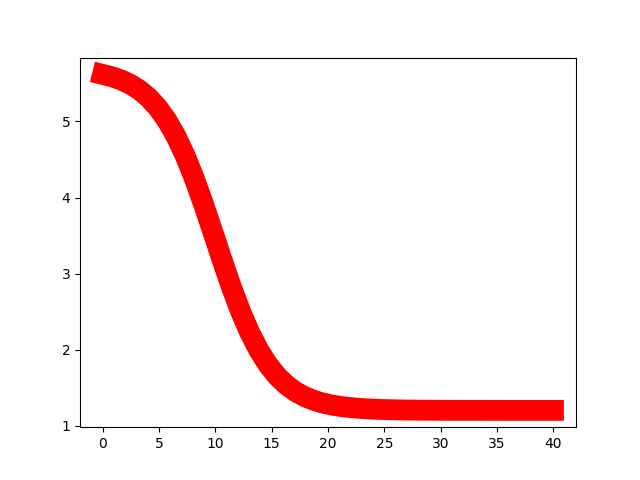
\includegraphics[scale=0.08, trim=70 70 70 0]{\outFolder/sig0.png}};
    \node  (traj) at (sig0.north) {\scriptsize{Traj. 0}}; 
     \node (sig1) at (2.75,2.25) {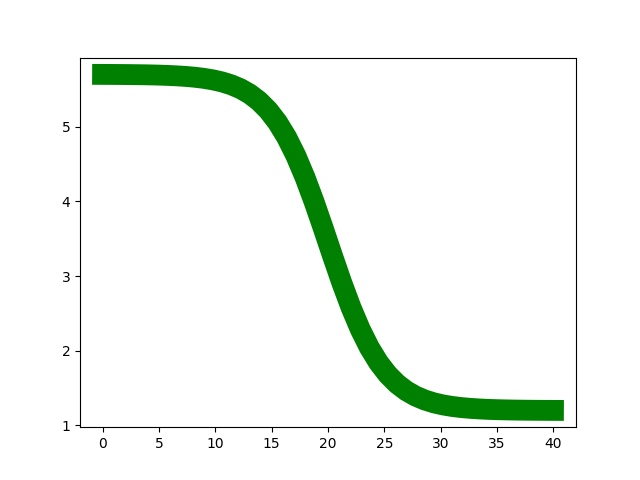
\includegraphics[scale=0.08, trim=70 70 70 0]{\outFolder/sig1.png}};
    \node  (traj) at (sig1.north) {\scriptsize{Traj. 1}}; 
     \node (sig2) at (3.00,0.80) {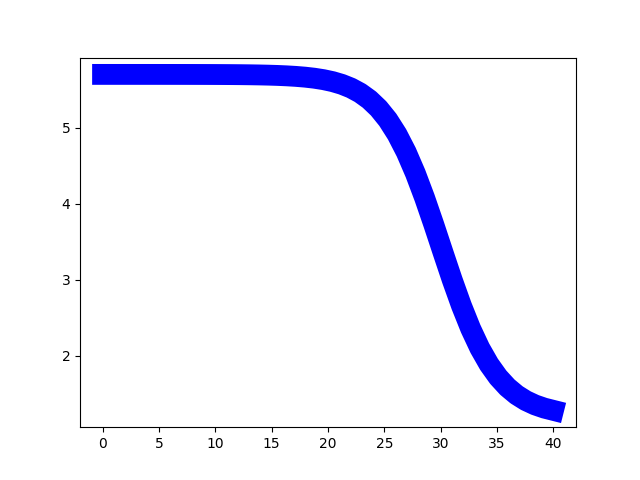
\includegraphics[scale=0.08, trim=70 70 70 0]{\outFolder/sig2.png}};
    \node  (traj) at (sig2.north) {\scriptsize{Traj. 2}}; 


    \draw[dotted, line width=0.6, color=red] (sig0.south west) -- (-0.1,1.5);
    \draw[dotted, line width=0.6, color=red] (sig0.south east) -- (1.8,1.5);

    \draw[dotted, line width=0.6, color=green] (sig1.west) -- (01,1.5);
    \draw[dotted, line width=0.6, color=green] (sig1.south) -- (1.8,0);

    \draw[dotted, line width=0.6, color=blue] (sig2.north west) -- (1.6,1.5);
    \draw[dotted, line width=0.6, color=blue] (sig2.south west) -- (0.7,0.3);

    \node  (vertices_label) at (0.8,1.8) {\scriptsize{Vertices}};


    % draw the bran and the magnification from it
    \node  (brain) at (1,-1.5) {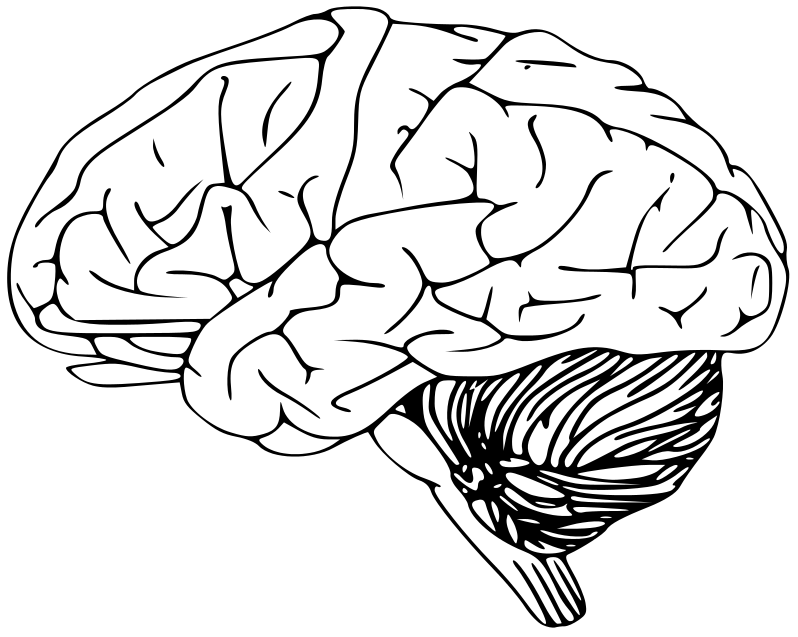
\includegraphics[scale=0.06]{\outFolder/brain.png}};

    \draw (1,-1.4) circle (0.15cm) node (C) {};
    \draw[line width=0.6, color=black] (C.west) -- (-0.1,0);
    \draw[line width=0.6, color=black] (C.east) -- (1.8,0);


   \end{tikzpicture}
  \end{figure}

    %\end{block}
    \end{column}
  \end{columns}
 
  
  \begin{equation}
\label{eq:dps_vwdpm6}
 p(V|\alpha, \beta, \theta, \sigma) = \prod_{l=1}^L \sum_{k=1}^K p(Z_l = k) \prod_{(i,j) \in I} N(V_l^{ij} | f(\alpha_i t_{ij} + \beta_i | \theta_k), \sigma_k)
\end{equation}

\vspace{-2em}

\end{frame}


\begin{frame}
\frametitle{Vertexwise Model - Fitting Procedure}

\newcommand{\lw}{0.5mm}
% \newcommand{\mycirc}[2]{\draw (#1,#2) circle (3cm);}

\newcommand{\outFolder}{.}
     
    \vspace{1em} 
    \textbf{Model fitting with EM}:
    \vspace{1em}
    \begin{itemize}
    \item \textbf{E-step}:
    \begin{itemize}
     \item Estimate vertex assignment to clusters:
     
     \begin{equation}
 z_{lk} =  \frac{\prod_{(i,j) \in I} N(V_l^{ij} | f(\alpha_i^{old} t_{ij} + \beta_i^{old} | \theta_k^{old}), \sigma_k^{old})}{\sum_{m=1}^K \prod_{i,j \in I} N(V_l^{ij} | f(\alpha_i^{old} t_{ij} + \beta_i^{old} | \theta_m^{old}), \sigma_m^{old})}
\end{equation}

    \end{itemize}
    \item \textbf{M-step}:
    \begin{itemize}
     \item Update trajectories:
     
     \begin{equation}
 \label{eq:theta}
 \theta_k = \argmin_{\theta_k} \left[\sum_{l=1}^L z_{lk} \sum_{(i,j) \in I} (V_l^{ij} - f(\alpha_i t_{ij} + \beta_i | \theta_k))^2 \right] - log\ p(\theta_k) 
\end{equation}
     
     \item Update subject stages:
     
     \begin{equation}
\label{eq:alpha}
 \alpha_i, \beta_i = \argmin_{\alpha_i, \beta_i}  \left[ \sum_{l=1}^L \sum_{k=1}^K z_{lk} \frac{1}{2\sigma_k^2} \sum_{j \in I_i} (V_l^{ij} - f(\alpha_i t_{ij} + \beta_i | \theta_k))^2\right] - log\ p(\alpha_i, \beta_i)
\end{equation}
     
    \end{itemize}
    \end{itemize}
    %\end{block}


\end{frame}


\begin{frame}
\frametitle{Vertexwise Model - Simulation Results}

\begin{itemize}
 \item Simulated data from 1,000 vertices generated from 3 clusters
 \item Recovered the (a) underlying trajectories and (b) subject stages
 \item Optimal number of clusters was estimated with BIC.
\end{itemize}


\newcommand{\imgFold}{../images/vwdpm}

\begin{figure}
\begin{subfigure}[b]{0.75\textwidth}
  \hspace{-1em}
  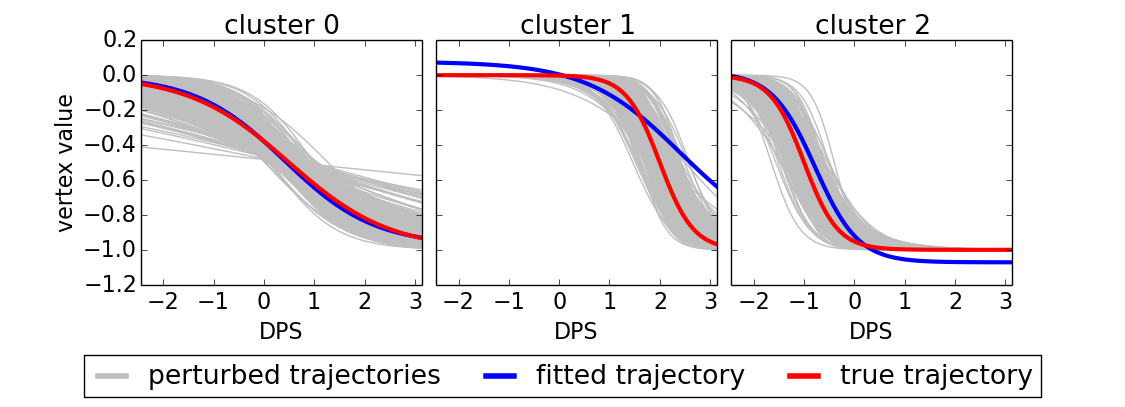
\includegraphics[width=1\textwidth]{\imgFold/synThetaRes_gensigInitk-meansCl3Pr1Ra0_VWDPMStd.png}
  \caption{}
  \label{fig:synThetaRes}
\end{subfigure}
\hspace{-2em}
\begin{subfigure}[b]{0.24\textwidth}
\centering
  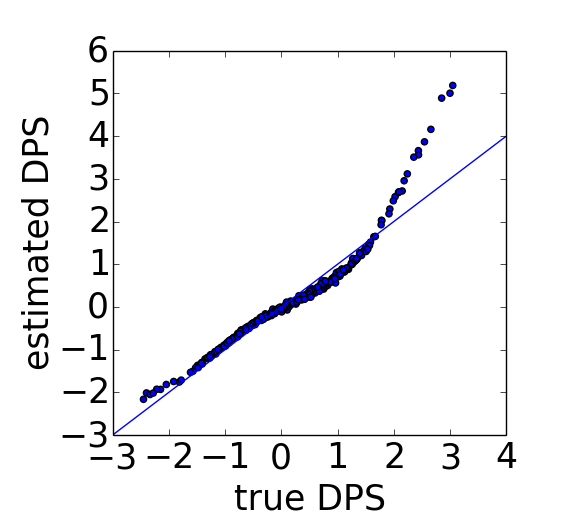
\includegraphics[width=1.1\textwidth]{\imgFold/synShiftsRes_gensigInitk-meansCl3Pr1Ra0_VWDPMStd.png}
  \vspace{0.9em}
  \caption{}
  \label{fig:synShiftRes}
\end{subfigure}
% \caption{Estimated (a) trajectories and (b) subject stages}
\end{figure}
\end{frame}

\begin{frame}
\frametitle{Datasets}

\textbf{ADNI}:
\begin{itemize}
 \item Used T1 MRI scans from 328 subjects (controls, MCI and AD)
 \item Average of 4.95 scans per subject
\end{itemize}

\vspace{2em}

\textbf{DRC}:
\begin{itemize}
 \item T1 scans from 31 healthy controls, 32 PCA and 24 tAD subjects.
 \item Average of 5.26 scans per subject
\end{itemize}

\vspace{2em}

\textbf{Preprocessing}:
\begin{itemize}
 \item Extracted veretexwise cortical thickness measurements with Freesurfer.
 \item Vertex measurements were standardised w.r.t. controls
\end{itemize}



\end{frame}


%%%%%%%%%%%%%%%%%%%%%%%%%%%%%%%%%%%%%%%%%%%%%%

\begin{frame}
\frametitle{Vertexwise Model - ADNI and DRC Results}

\newcommand{\scalingFactor}{0.4}

\newcommand{\gradLimLeft}{-1.6}
\newcommand{\gradLimRight}{1.6}

% \newcommand{\scalingFactorLeftFig}{1.2}
\newcommand{\scalingFactorBrains}{0.9}
\newcommand{\scalingFactorTraj}{1}

% FWHM0 avg thickness map MCI & AD
\begin{figure}[h]
  \centering

  % do the legend colorbar
  \begin{subfigure}[b]{\textwidth}
   \centering
  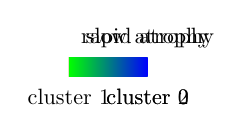
\begin{tikzpicture}[scale=1, every node/.style={scale=0.8}]
    \shade[left color=red,right color=green] (\gradLimLeft,2.5) rectangle (0,2.75);
    \shade[left color=green,right color=blue] (0,2.5) rectangle (\gradLimRight,2.75);
    \node[inner sep=0] (corr_text) at (\gradLimLeft,2.25) {cluster 0};
    \node[inner sep=0] (corr_text) at (0,2.25) {cluster 1};
    \node[inner sep=0] (corr_text) at (\gradLimRight,2.25) {cluster 2};
    \node[inner sep=0] (corr_text) at (\gradLimLeft,3) {rapid atrophy};
    \node[inner sep=0] (corr_text) at (\gradLimRight,3) {slow atrophy};
  \end{tikzpicture}
%     \caption{}
%       \label{fig:adniClust}
  \vspace{1em}
  \end{subfigure}
  
  %%%%%%%%%%%%%%%%%%% BRAINS %%%%%%%%%%%%%%5%%%%%%
  
  \begin{subfigure}[b]{0.3\textwidth}
   \centering
  \begin{tikzpicture}[scale=\scalingFactor, every node/.style={scale=1}]
    \node[inner sep=0] (image) at (0,0) {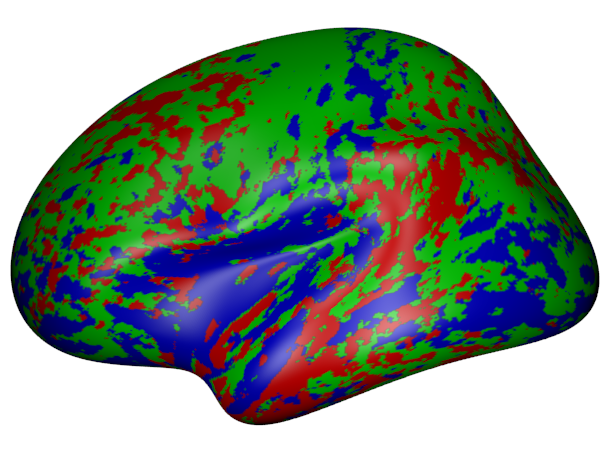
\includegraphics[width=\scalingFactorBrains\textwidth]{../images/vwdpm/blend14_adniThavgFWHM0InithistCl3Pr0Ra1_VWDPMStd.png}}; 
    \node[inner sep=0] (label) at (0,3.5) {tAD - ADNI};
  \end{tikzpicture}
%     \caption{}
%       \label{fig:adniClust}
  \end{subfigure}
   \begin{subfigure}[b]{0.3\textwidth}
  \centering
  \begin{tikzpicture}[scale=\scalingFactor, every node/.style={scale=1}]
    \node[inner sep=0] (corr_text) at (0,0) {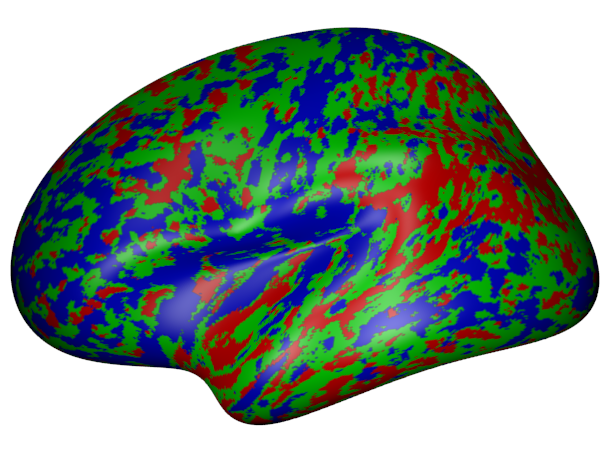
\includegraphics[width=\scalingFactorBrains\textwidth]{../images/vwdpm/drcThavgFWHM0InithistCl3Pr0Ra1_VWDPMStdAD_blend24.png}};
    \node[inner sep=0] (label) at (0,3.5) {tAD - DRC dataset};
  \end{tikzpicture}
%     \caption{}
%       \label{fig:drcClustAD}
  \end{subfigure}
   \begin{subfigure}[b]{0.3\textwidth}
  \centering
  \begin{tikzpicture}[scale=\scalingFactor, every node/.style={scale=1}]
    \node[inner sep=0] (corr_text) at (0,0) {\includegraphics[width=\scalingFactorBrains\textwidth]{../images/vwdpm/drcThavgFWHM0InithistCl3Pr0Ra1_VWDPMStdPCA_blend24.png}};
    \node[inner sep=0] (label) at (0,3.5) {PCA - DRC dataset};
  \end{tikzpicture}
%     \caption{}
%       \label{fig:drcClustPCA}
  \end{subfigure}
  
  %%%%%%%%%%%%%%%%%%%%%% trajectories %%%%%%%%%%%%%%%%%%%%%%%
  
    \begin{subfigure}[b]{0.3\textwidth}
    \centering
%     \vspace{-2em}
    \includegraphics[width=\scalingFactorTraj\textwidth]{../images/vwdpm/trajSamplesOneFig_adniThavgFWHM0InithistCl3Pr0Ra1_VWDPMStd.png}
%     \caption{}
%       \label{fig:adniTraj}
  \end{subfigure}
      \begin{subfigure}[b]{0.3\textwidth}
    \centering
%     \vspace{-2em}
    \includegraphics[width=\scalingFactorTraj\textwidth]{../images/vwdpm/trajSamplesOneFig_drcThavgFWHM0InithistCl3Pr0Ra1_VWDPMStdAD.png}
%     \caption{}
%       \label{fig:drcTrajAD}
  \end{subfigure}
    \begin{subfigure}[b]{0.3\textwidth}
    \centering
%     \vspace{-2em}
    \includegraphics[width=\scalingFactorTraj\textwidth]{../images/vwdpm/trajSamplesOneFig_drcThavgFWHM0InithistCl3Pr0Ra1_VWDPMStdPCA.png}
%     \caption{}
%       \label{fig:drcTrajPCA}
  \end{subfigure}
  
%   \caption{}
%   \label{fig:clustTrajAll}

\end{figure}

\textbf{Conclusion}: We can see a fine-grained spatial distribution of atrophy.

\end{frame}

\begin{frame}
\frametitle{Vertexwise Model - Validation of Estimated Clusters}

\newcommand{\outFoldADNICVbrains}{../../voxelwiseDPM/ipmi_paper/figures/crossvalid/adniThavgFWHM0Initk-meansCl3Pr0Ra1_VWDPMMean}

\newcommand{\scaleFig}{0.16}

\textbf{Cross-validation}
\begin{itemize}
 \item Tested the consistency of the spatial clustering across 10-fold CV
 \item Results show good agreement in terms of spatial distribution
 \item Average dice score overlap for each cluster pair: 0.89-0.90
\end{itemize}


\begin{figure}[h]
    \centering
    
    \begin{subfigure}[b]{\scaleFig\textwidth}\includegraphics[width=\textwidth]{\outFoldADNICVbrains/blend0.png}\end{subfigure}
    \begin{subfigure}[b]{\scaleFig\textwidth}\includegraphics[width=\textwidth]{\outFoldADNICVbrains/blend1.png}\end{subfigure}
    \begin{subfigure}[b]{\scaleFig\textwidth}\includegraphics[width=\textwidth]{\outFoldADNICVbrains/blend2.png}\end{subfigure}
    \begin{subfigure}[b]{\scaleFig\textwidth}\includegraphics[width=\textwidth]{\outFoldADNICVbrains/blend3.png}\end{subfigure}
    \begin{subfigure}[b]{\scaleFig\textwidth}\includegraphics[width=\textwidth]{\outFoldADNICVbrains/blend4.png}\end{subfigure}
    
    \begin{subfigure}[b]{\scaleFig\textwidth}\includegraphics[width=\textwidth]{\outFoldADNICVbrains/blend5.png}\end{subfigure}
    \begin{subfigure}[b]{\scaleFig\textwidth}\includegraphics[width=\textwidth]{\outFoldADNICVbrains/blend6.png}\end{subfigure}
    \begin{subfigure}[b]{\scaleFig\textwidth}\includegraphics[width=\textwidth]{\outFoldADNICVbrains/blend7.png}\end{subfigure}
    \begin{subfigure}[b]{\scaleFig\textwidth}\includegraphics[width=\textwidth]{\outFoldADNICVbrains/blend8.png}\end{subfigure}
    \begin{subfigure}[b]{\scaleFig\textwidth}\includegraphics[width=\textwidth]{\outFoldADNICVbrains/blend9.png}\end{subfigure}
    
%     \caption{Cross-validation}
    \label{fig:ADNICVbrains}
\end{figure}

\end{frame}

\begin{frame}
\frametitle{Vertexwise Model - Validation of Stages}

\textbf{Staging validation}
\begin{itemize}
 \item Tested consistency of stages of subjects across different visits
 \item 84\% of subjects analysed show increasing stages over time
 \item Stages correlate well with cognitive tests:
 \begin{itemize}
  \item CDRSOB ($\rho = 0.41$, $p < 1e-66$)
  \item ADAS-COG ($\rho = 0.40$, $p < 1e-62$)
  \item MMSE ($\rho = 0.39$, $p < 1e-58$) 
 \end{itemize}
\end{itemize}

\vspace{-1em}

\begin{figure}[h]
    \centering
    \includegraphics[width=0.5\textwidth]{../../voxelwiseDPM/ipmi_paper/figures/crossvalid/stagingConsist_adniThavgFWHM0Initk-meansCl3Pr0Ra1_VWDPMMean.png}
%     \caption{The disease progression score for each subject from the ADNI dataset estimated during 10-fold cross validation. Each line represents an individual $i$ with different visits $j$. Later visits generally have a higher corresponding stage.}
%     \label{fig:stagingConsist}
\end{figure}

\vspace{-2em}

\end{frame}


\begin{frame}
\frametitle{Future Work Plan}

% \tikzset{every picture/.append style={scale=2.5}}

% Gantt chart
\begin{figure}

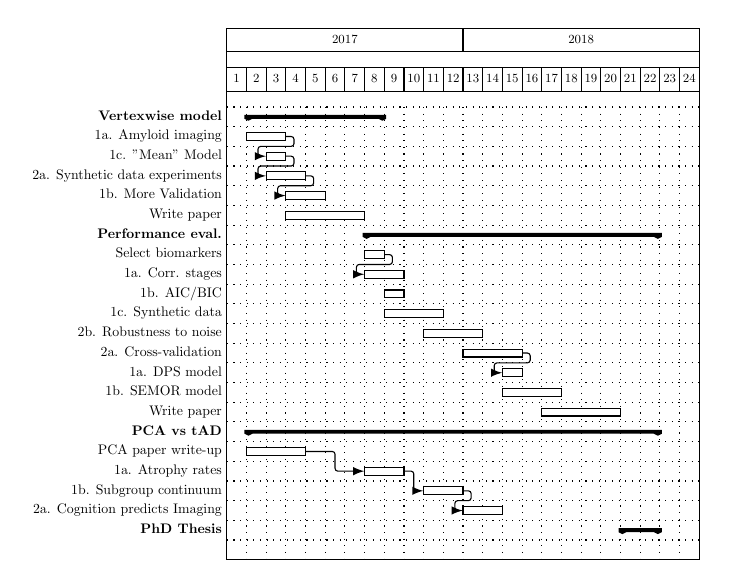
\begin{tikzpicture}[scale=0.5, every node/.style={scale=0.5}]
\begin{ganttchart}[vgrid, hgrid,y unit chart=0.5cm]{1}{24}
\gantttitle{2017}{12}
\gantttitle{2018}{12}\\
\gantttitlelist{1,...,24}{1}\\
%First Group
\ganttgroup{Vertexwise model}{2}{8} \\
\ganttbar{1a. Amyloid imaging}{2}{3} \\
\ganttbar{1c. "Mean" Model}{3}{3}\\
\ganttbar{2a. Synthetic data experiments}{3}{4}\\
\ganttbar{1b. More Validation}{4}{5} \\
\ganttbar{Write paper}{4}{7}\\
%\ganttlink{elem0}{elem1}
\ganttlink{elem1}{elem2}
\ganttlink{elem2}{elem3}
\ganttlink{elem3}{elem4}
% \ganttlink{elem4}{elem5}
%\ganttmilestone{Milestone 1}{11}
%Second Group
\ganttgroup{Performance eval.}{8}{22} \\
\ganttbar{Select biomarkers}{8}{8} \\
\ganttbar{1a. Corr. stages}{8}{9} \\
\ganttbar{1b. AIC/BIC}{9}{9} \\
\ganttbar{1c. Synthetic data}{9}{11}\\
\ganttbar{2b. Robustness to noise}{11}{13}\\
\ganttbar{2a. Cross-validation}{13}{15}\\
\ganttbar{1a. DPS model}{15}{15}\\
\ganttbar{1b. SEMOR model}{15}{17}\\
\ganttbar{Write paper}{17}{20}\\

\ganttlink{elem7}{elem8}
\ganttlink{elem12}{elem13}
%\ganttmilestone{Milestone 1}{11}
%Third Group
\ganttgroup{PCA vs tAD}{2}{22} \\
\ganttbar{PCA paper write-up}{2}{4}\\
\ganttbar{1a. Atrophy rates}{8}{9}\\
\ganttbar{1b. Subgroup continuum}{11}{12}\\
\ganttbar{2a. Cognition predicts Imaging}{13}{14}\\

\ganttlink{elem17}{elem18}
\ganttlink{elem18}{elem19}
\ganttlink{elem19}{elem20}

\ganttgroup{PhD Thesis}{21}{22} \\


\end{ganttchart}
\end{tikzpicture}
\end{figure}

\end{frame}

% \begin{frame}
% \frametitle{Acknowledgements}
% 
% \begin{figure}
%  \begin{subfigure}{0.32\textwidth}
%  \centering
%  Daniel Alexander
%  \includegraphics[scale=0.35]{Danny-Alexander.jpeg}  
%  \end{subfigure}
%   \begin{subfigure}{0.32\textwidth}
%   \centering
%   Sebastian Crutch
%  \includegraphics[scale=0.35]{Seb_Crutch_photo.JPG}  
%  \end{subfigure}
%   \begin{subfigure}{0.32\textwidth}
%   \centering
%   Timothy Shakespeare
%  \includegraphics[scale=0.2]{tim_photo.png}  
%  \end{subfigure}
%  \vspace{1em}
%  
%   \begin{subfigure}{0.25\textwidth}
%  \centering
%  Neil Oxtoby
%  \includegraphics[scale=0.35]{neil_photo.jpg}  
%  \end{subfigure}
%   \begin{subfigure}{0.25\textwidth}
%  \centering
%  Alexandra Young
%  \includegraphics[scale=0.5]{alex_photo.jpg}  
%  \end{subfigure}
%   \begin{subfigure}{0.3\textwidth}
%   \centering
%   \includegraphics[scale=0.15]{CDTlogo.png}\\
%   \vspace{1em}
%   \includegraphics[scale=1]{pondLogo.png}  
%   \end{subfigure}
% 
% \end{figure}
% 
% 
% \end{frame}

 
\end{document}

